\chapter{Tonotactics} 
\label{chap:tonotactics}


\section{Introduction}\label{sec:intro} 
This paper provides one
method for learning tonotactic patterns over autosegmental
representations (ARs). A key insight of phonological theory is to view
forms in tonal languages as \textit{autosegmental graphs}, rather than
one-dimensional linear strings \citep{goldsmith1976autosegmental,
	coleman1991no, jardine2017LocalNature,
	oakdenNotationalEquivalenceTonal2020}. These representations have
been argued to offer advantages for analysing tonal
patterns \citep{hyman2009representation, clements2010autosegmental,
	oddenintroducing2013}.  Computationally, grammars over ARs have been
shown to express both local and long-distance constraints, while
maintaining a relatively low level of computational complexity
\citep{jardine2017LocalNature, chandleejardine19aisl}.  
However, despite the importance of ARs in tonal phonology and previous research
on their formal properties \citep{kornai2007mathematical},  
there has been limited work on learning tonal grammars, and, to our 
knowledge, no phonotactic learning models have adopted ARs.

This paper focuses on learning tonotactic grammars. Following
\citet{jardine2017LocalNature}, the tonotactic grammar consists of a
set of language-specific inviolable constraints over ARs. The
constraints themselves only specify marked AR structures. Logically,
such grammars are simply the conjunction of negative literals
\citep{rogers.lambert2019mol}. In this setting, the tonotactic
learning problem boils down to identifying those constraints (the
marked AR structures) which are consistent with the entire dataset.

The Bottom-Up Factor Inference Algorithm (BUFIA) is a learning
algorithm that deterministically searches a space of possible
constraints and is provably guaranteed to find the most general
constraints consistent with its input data \citep{chandleeBufia2019,
	rawski2021structure}. Crucially, it is couched in model theory
\citep{Rogers1998, enderton2001mathematical} so that it can operate
with any particular representational scheme.

This work presents BUFIA-AR, an instantiation of BUFIA that learns
tonotactic constraints expressed with ARs. As will be explained, this
implementation utilises a matrix-based representation for ARs, which
is an adaptation of matrix-based representations of graphs
\citep{west2001introduction,CLRS2022}.

BUFIA-AR was tested on a curated corpus of Hausa \citep{wold-4,li2025learning}, a
Chadic language in West Africa. The corpus consists of 621
mono-morphemic words, which altogether provide a collection of 64
distinct ARs.  Using this corpus as input, we assess the performance
of BUFIA-AR through a combination of qualitative and quantitative
evaluations. Qualitatively, BUFIA-AR returns a grammar
consisting of 11 AR constraints when syllable, tone, and mora counts
are limited to three. These BUFIA-AR-learned constraints either align
with, or are more specific than, those previously proposed in the
literature. The algorithm additionally identifies novel patterns that
have not been previously reported. Quantitatively, a cross-validation
experiment shows that BUFIA-AR achieves a mean accuracy over 90\% in
both token- and type-based settings, which outperforms the linguistic 
baseline grammar and a BUFIA learner using
string representations (BUFIA-Str). Altogether, these results
demonstrate the feasibility of using BUFIA-AR for tonotactic grammar
inference. All data and programs used in this paper are accessible in
the Dryad repository.

In this way, this paper takes a first step towards learning tonal
grammars expressed in terms of ARs. We acknowledge that tonal grammars
are much more than just the tonotactic component. The grammars that
BUFIA-AR returns have nothing to say about how underlying
representations of tonal languages are learned, nor how these
underlying representations are transformed into surface
representations. We also acknowledge that some surface constraints
have been argued to follow from the tonal processes themselves in some
languages (see Section~\ref{sec:learning}), which is again something
the grammars returned by BUFIA-AR cannot express. Nonetheless, despite
these limitations, BUFIA-AR still makes a contribution to our
understanding of how tonal grammars expressed in terms of ARs can be
learned. We expect that some of the insights made here will persist in
future research which addresses these broader problems regarding the
learning of tonal grammars.

This paper is structured as follows. Section~\ref{sec:learning}
provides an overview of the tonotactic learning problem and current models. Section~\ref{sec:prelim} introduces 
formal language theory, model theory, and graph theory relevant to ARs
and BUFIA. Section~\ref{sec:bufiaar} provides a detailed description
of the BUFIA-AR implementation. Section~\ref{sec:hausa} presents the Hausa case study and model evaluations. Section~\ref{sec:discussion}
discusses issues relating to constraint optimisation, constraint
satisfaction, and constraint weighting. Section~\ref{sec:conclusion}
concludes the paper and points to some future directions.


\section{Learning Tonotactics} \label{sec:learning}
\subsection{Tonal Mapping Problem}\label{sec:learning.mapping}

A central question in tonal phonology concerns how languages organise 
tones, syllables, and/or moras into well-formed structures. A 
closely related modelling question asks what kinds of well-formed 
tonal patterns are attested in a language, and how such patterns 
can be systematically characterised. To illustrate these issues, 
we begin with a frequently discussed example: the tonal mapping 
problem in two West African tonal languages, Hausa and Mende. 
Hausa is a Chadic language, while Mende is a Southwestern Mande 
language spoken in Sierra Leone \citep{lebenRepresentationTone1978}.
Both languages use High (H) and
Low (L) tones as basic tonemes with the mora as the tone-bearing unit
(TBU). However, they show distinct patterns in how their tonal
melodies are mapped to TBUs \citep{Newmanbook,
	lebenRepresentationTone1978, zoll2003optimal, jardine2017LocalNature}.  

  
As shown in Table~\ref{tab.hausa.mende}, the two languages first differ in their
monosyllabic contour inventory. Mende permits a wider range of monosyllabic contours, including 
light HL, heavy HL, and heavy LH, whereas Hausa allows only the heavy HL contour. 
Secondly, when a two-tone melody maps onto a trisyllabic word, Mende and 
Hausa have distinct surface forms: 
HL surfaces as H.L.L in Mende (\textit{fé.là.là} `junction') but as H.H.L in Hausa 
(\textit{jée.máa.gèe} `bat'); similarly, LH surfaces as L.L.H in Mende 
(\textit{lè.lè.má} `mantis') but as L.H.H in Hausa (\textit{jì.mí.ná} 
`ostrich')\footnote{This
	paper follows the
	tonal transcription method commonly used by Africanists. For
	instance, ``H.H.L'' represents two H-toned syllables followed 
	by a L-toned syllable. In addition, tones are always
	marked on the nuclear vowels. Long
	vowels are transcribed as double vowels.}\(^,\)\footnote{\citet{dwyerMende1978} offers a different
	analysis of Mende tones than \citet{lebenRepresentationTone1978}'s,
	and provides supplemental data in which L.H.H forms also occur (e.g.
	\textit{ndàvúlá} `sling'). \citet{lebenRepresentationTone1978}
	account for the different patterns by proposing two distinct
	mappings.}.

\begin{table}
	\centering
	\begin{tabular}
		{
			>{\centering\arraybackslash}m{1.35cm}|
			>{\centering\arraybackslash}m{4.5cm}|
			>{\centering\arraybackslash}m{4.5cm}
		}
\toprule
		& Mende & Hausa \\
\midrule
		contour inventory
		&
		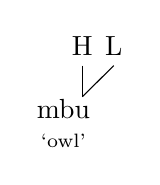
\begin{tikzpicture}[scale=.8]
			
			\node (seg) at (0,0) {mbu};
			\node[font=\scriptsize] at (0,-0.5) {`owl'};
			\node (H) at (0.3,1) {H};
			\node (L) at (0.8,1) {L};
			\coordinate (v) at (0.3,0.2);
			\draw (H.south) -- (v);
			\draw (L.south) -- (v);
		\end{tikzpicture}\hfil
		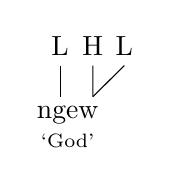
\begin{tikzpicture}[scale=.8]
	
			\node (seg) at (0,-.1) {ngew\textopeno\textopeno};
			\node[font=\scriptsize] at (0,-0.5) {`God'};
			
			\node (T1) at (-0.12,1) {L};
			\node (T2) at (0.4,1) {H};
			\node (T3) at (0.9,1) {L};
			
			\coordinate (a1) at (-0.12,0.2);
			\coordinate (a2) at ( 0.4,0.2);
			
			\draw (T1) -- (a1);
			\draw (T2) -- (a2);
			\draw (T3.south) -- (a2);
		\end{tikzpicture} \hfil
		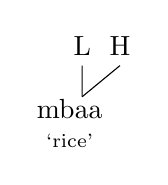
\begin{tikzpicture}[scale=.8]
			\node (c) at (0,0) {mbaa};
			\node[font=\scriptsize] at (0,-0.5) {`rice'};
			\node (t1) at (0.2,1) {L};
			\node (t2) at (0.8,1) {H};
			\draw (t1) -- (0.2,0.2);
			\draw (t2.south) -- (0.2,0.2);
		\end{tikzpicture} 
		&
		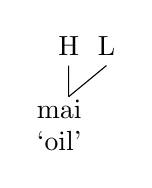
\begin{tikzpicture}[scale=.8]
			\node (c) at (0,0) {mai};
			\node (g) at (0,-0.5) {`oil'};
			\node (t1) at (0.15,1) {H};
			\node (t2) at (0.75,1) {L};
			\draw (t1) -- (0.15,0.2);
			\draw (t2.south) -- (0.15,0.2);
		\end{tikzpicture} \\ \midrule
		tone mapping 
		&
		\begin{tikzpicture}[scale=.8]
			\node (c) at (0,0) {f e l a l a};
			\node (g) at (0,-0.5) {`junction'};
			\node (t1) at (-0.4,1) {H};
			\node (t2) at (0.13,1) {L};
			\draw (t1) -- ($(t1.south)+(0,-.45)$);
			\draw (t2) -- ($(t2.south)+(0,-.45)$);
			\draw (t2.south) -- ($(t2.south)+(.5,-.45)$);
		\end{tikzpicture} \hfil
		\begin{tikzpicture}[scale=.8]
			\node (c) at (0,0) {l e l e m a};
			\node (g) at (0,-0.5) {`mantis'};
			\node (t1) at (0,1) {L};
			\node (t2) at (0.75,1) {H};
			\draw (t1.south) -- ($(t1.south)+(0,-.45)$);
			\draw (t1.south) -- ($(t1.south)+(-.5,-.45)$);
			\draw (t2.south) -- ($(t2.south)+(0,-.45)$);
		\end{tikzpicture}
		&
		\begin{tikzpicture}[scale=.8]
			\node (c) at (0,0) {j ee m aa g ee};
			\node (g) at (0,-0.5) {`bat'};
			\node (t1) at (.1,1) {H};
			\node (t2) at (0.9,1) {L};
			\draw (t1.south)-- ($(t1.south)+(0,-.45)$);
			\draw (t1.south)-- ($(t1.south)+(-0.9,-.45)$);
			\draw (t2.south) -- ($(t2.south)+(0,-.45)$);
		\end{tikzpicture} \hfill
		\begin{tikzpicture}[scale=.8]
			\node (c) at (0,0) {j i m i n a};
			\node (g) at (0,-0.5) {`ostrich'};
			\node (t1) at (-0.55,1) {L};
			\node (t2) at (0.12,1) {H};
			\draw (t1) -- ($(t1.south)+(0,-.4)$);
			\draw (t2.south) -- ($(t2.south)+(0,-.4)$);
			\draw (t2.south) -- (0.7,0.2);
		\end{tikzpicture}\\
	\bottomrule
	\end{tabular}
	\caption{Contour inventories and tone mapping in Mende and Hausa.}
	\label{tab.hausa.mende}
\end{table}


There are mainly three approaches to the tone mapping problem. The
first identifies three key factors that determine the surface forms:
\textit{directionality} (whether tone spreads rightwards or leftwards), 
\textit{morphological categories }(prefix or suffix), and \textit{tone quality}
(whether spreading is sensitive to H or L) \citep{hyman1987prosodic,
	leben2017tone, hyman2009representation}.

The second account is Optimal Tone Mapping \citep[OTM;][]
{zoll2003optimal}. Zoll argues that directionality-based accounts of
phonological mapping can in some cases yield incorrect surface
predictions. Under OTM, surface tonal patterns emerge from
language-specific rankings between morphological faithfulness
constraints and markedness constraints, \textsc{Clash} and
\textsc{Lapse}, which are sensitive to tone quality.

The third approach, proposed by \citet{jardine2017LocalNature}, 
is to use language-specific, inviolable constraints, where the
constraints are marked, forbidden ARs; that is, ARs to be
avoided. For example, the \textsc{No Short Rise} constraint in Mende
\citep{leben2017tone} that forbids the monomoraic syllable with a LH 
melody can be represented as in Figure~\ref{graph:lh1}.

\begin{figure}[ht]
	\centering
	% --- subtable 1 ---
	\begin{minipage}[b]{0.25\textwidth}
		\centering
		\begin{tikzpicture}
			\node (neg) at (-0.8,2) {\Large $\neg$};		
			\node [] (t1) at (0,2) {L};
			\node [] (t2) at (0.6,2) {H};            
			\node [] (c1) at (0,1) {$\mu$};
			\node [] (s1) at (0,0) {$\sigma$};
			\draw [-] (t1) to (c1.north);
			\draw [-] (t2.south) to (c1.north);
			\draw (c1) -- (s1);
		\end{tikzpicture}
		\subcaption{*$\check{\mu}$}
		\label{graph:lh1}
	\end{minipage}
	\hfill
	% --- subtable 2 ---
	\begin{minipage}[b]{0.25\textwidth}
		\centering
		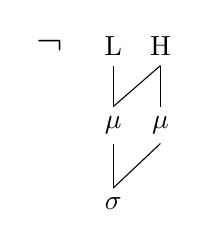
\begin{tikzpicture}
			\node (neg) at (-0.8,2) {\Large $\neg$};
			\node [] (t1) at (0,2) {L};
			\node [] (t2) at (0.6,2) {H};            
			\node [] (c1) at (0,1) {$\mu$};
			\node [] (c2) at (0.6,1) {$\mu$};
			\node [] (s1) at (0,0) {$\sigma$};
			\draw [-] (t1) to (c1.north);
			\draw [-] (t2.south) to (c1.north);
			\draw [-] (t2.south) to (c2.north);
			\draw [-] (c1.south) to (s1.north);
			\draw [-] (c2.south) to (s1.north);
		\end{tikzpicture}
		\subcaption{*$\check{\mu}\acute{\mu}$}
		\label{graph:lh2}
	\end{minipage}
	\hfill
	% --- subtable 3 ---
	\begin{minipage}[b]{0.3\textwidth}
		\centering
		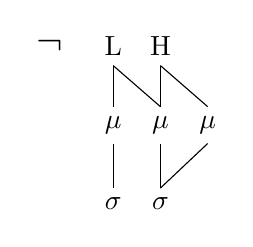
\begin{tikzpicture}
			\node (neg) at (-0.8,2) {\Large $\neg$};
			\node [] (t1) at (0,2) {L};
			\node [] (t2) at (0.6,2) {H};
			\node [] (c1) at (0,1) {$\mu$};
			\node [] (c2) at (0.6,1) {$\mu$};
			\node [] (c3) at (1.2,1) {$\mu$};
			\node [] (s1) at (0,0) {$\sigma$};
			\node [] (s2) at (0.6,0) {$\sigma$};
			\draw (t1.south) -- (c1.north);
			\draw (c1.south) -- (s1.north);
			\draw (t1.south) -- (c2.north);
			\draw (c2.south) -- (s2.north);
			\draw (t2.south) -- (c3.north);
			\draw (c3.south) -- (s2.north);
			\draw (t2.south) -- (c2.north);
		\end{tikzpicture}
		\subcaption{*$\grave{\mu}\check{\mu}\acute{\mu}$}
		\label{graph:lh3}
	\end{minipage}
	\hfill
\caption{The forbidden structure in (a), *$\check{\mu}$ (corresponding to \textsc{No Short Rise}), and two ARs in (b--c) containing it.}	\label{intro.fig.noLH}
\end{figure}

Following \citet{jardine2017LocalNature}, if
Figure~\ref{graph:lh1} is forbidden in the language, any AR
\textit{containing} it, such as
Figure~\ref{graph:lh2}-\ref{graph:lh3}, will also be
forbidden. Formally, if Grammar $G$ is the set of constraints in the
language, such that \(G = \{AR_1, AR_2, \ldots, AR_n\}\), a well-formed
AR satisfies the \emph{conjunctive negative literals}:
\(\lnot AR_1 \land \lnot AR_2 \land \ldots \land \lnot AR_n\)
\citep{jardine2017LocalNature,rogers.lambert2019mol}. It follows that
the tonotactic learning problem is to identify a set \(G\) of banned
ARs given a set of example surface forms. This paper follows the third
approach of \citet{jardine2017LocalNature}.  


One potential criticism of \citet{jardine2017LocalNature}, anticipated
by the author and also applicable to the present work, is that it
explains tonal patterns exclusively in terms of surface-true
constraints. One consequence is that well-formed patterns that are not
directly observable in surface forms, or at the lexical level, are not
realised by the grammar. The grammar inferred at this level therefore
reflects only the final outcomes of tonal mapping, rather than
intermediate representations produced by tonal rules, which
potentially misses important phonological generalisations.

Hausa provides a clear illustration of this point. The absence 
of rising tones on a single syllable can be explained as follows. 
An underlying LH sequence may arise as an intermediate representation, 
either through synchronic processes or as the result of 
historical change, but it is subsequently simplified to either H in non-final 
position or L elsewhere \citep{Leben,Newmanbook}. Likewise, the absence of final 
L.L sequences on long vowels is attributed to \textsc{Low Tone Raising}, which 
changes underlying L.L to L.H when the second L occurs on a long vowel \citep{Leben,leben1996tonal}.

This example illustrates that unattested surface patterns do not
necessarily reflect illicit structures in the grammar itself, but
rather intermediate representations that are subsequently subject to
some repair processes. While acknowledging the limitations of these
grammars, we argue that learning such grammars is nonetheless
valuable. They still provide meaningful insights into tonotactic
patterns and serve as a foundation for further work for three reasons.

First, a grammar containing a set of forbidden ARs that is consistent
with observable surface forms is not in conflict with a grammar for
the tonal processes; rather, it captures their pronounceable
outcomes. Given available access to a lexicon at a
different level of abstractness, another grammar could likewise be
learned, and these two grammars can be systematically compared. This
comparison between different levels of abstractness itself yields
non-trivial insights into tonal processes.

Second, considering that ARs have been long used in tonal phonology, 
yet are absent from computational learning, we believe a more pressing 
priority is establishing representational adequacy for learning tones, 
which is the goal of this work.
Without an explicit framework
that encodes the geometry of tonal representations, modelling more
complex tonal alternations, such as those discussed above, is more
difficult. Establishing this representational foundation is therefore
a useful precondition for future work on deeper tonal processes.

Lastly, we are not aware of existing learning models that operate
with ARs directly for either tonal processes or tonotactics. In the next
section, we review previous learning approaches related to tier-based
representations and learning, and then introduce BUFIA, the algorithm
that our model is based on.

\subsection{Learning Models}\label{sec:learning.models}

This section reviews systems for phonotactic and tonotactic
learning. One line of research employs statistical methods from
machine learning \citep{CP97, hayes2008maximum,
	goldsmith2012information}. These methods have
been deployed on string and syllabic representations for learning
segmental phonotactic patterns as well as stress patterns,
but have not been used for learning tonotactics with ARs.

\citet{GouskovaGallagher2020} synthesises the Maximum Entropy (MaxEnt)
strategy of \citet{hayes2008maximum} with a procedure that induces
phonological tiers in order to learn non-local phonotactics. Related
work by
\citeauthor{Jardine-Heinz-2016-LTSLL}~(\citeyear{Jardine-Heinz-2016-LTSLL}),
\citeauthor{jardinemcmullin17}~(\citeyear{jardinemcmullin17}),
\citeauthor{de-santo-aksenova-2021-learning}~(\citeyear{de-santo-aksenova-2021-learning}),
and
\citeauthor{pmlr-v153-lambert21a}~(\citeyear{pmlr-v153-lambert21a}),
and \citeauthor{Swanson2025}~(\citeyear{Swanson2025}) provide
theoretical results and algorithms regarding the induction of
phonological tiers for non-local phonotactics. Other work has proposed
procedures for learning tiers for grammars modelling non-local
phonological processes \citep{BurnessMcMullin2019,
	burness-mcmullin-2021, Belth2024}. While the successful induction of
tiers from data is an important achievement of the 21st century, the
constraints induced over the projected tiers are still strings, and
not ARs. For example, none of the aforementioned methods can learn a
constraint that describes a many-to-one association from the tonal
tier to the TBU tier or vice versa.

BUFIA represents another approach \citep{chandleeBufia2019, rawski2021structure}.
BUFIA differs from the aforementioned approaches in a couple of ways. First,
it is not specific to any particular representation or data structure,
such as strings or trees. For this reason,
\citeauthor{chandleeBufia2019}'s (\citeyear{chandleeBufia2019})
presentation of BUFIA abstracts away from a specific representation,
and presents BUFIA in terms of arbitrary model-theoretic relational
structures. As long as the representations of interest can be
expressed model-theoretically, BUFIA can be implemented. %Consequently,
Since strings, trees, and graphs are all examples of structures that
have model-theoretic representations, versions of BUFIA can in
principle be designed for finding constraints over any of these
representations. This generality not only allows it to be
instantiated and ultimately deployed for the learning of a variety of
constraint types, but it also makes clear how the structure of the
space of possible constraints facilitates learning.

Second, BUFIA is a deterministic learning algorithm and in its current
form uses no statistical methods or randomness in its decision-making.
Basically, BUFIA checks possible constraints against the data one at a
time, adding those that are consistent with the data. It returns a
grammar consisting of inviolable constraints. As such, this grammar is
a conjunction of negative literals:
$\lnot C_1 \land \lnot C_2 \land \ldots \land \lnot C_n$, where each
\(C_i\) is a constraint, that is, a forbidden relational structure.

As will be explained in Section~\ref{sec:prelim.bufia}, BUFIA works because
any representational scheme orders the expressible constraints in a
natural way. By beginning with the smallest constraint, BUFIA is
guaranteed to search as much of the space as possible and return the
most general constraints (that is, the smallest forbidden structures)
consistent with the data, before a stopping condition is
met. Furthermore, BUFIA has been shown to be at least as successful in
learning feature-based, segmental phonotactics of Quechua
\citep{Swanson+2025} as phonotactic learning models based on the
principle of Maximum Entropy \citep{hayes2008maximum,
	wilson2018accidental}. However, BUFIA has not previously been used
in tonotactic learning over non-string representations.

To sum up, while ARs have long been conceptualised as graph
structures, no existing work learns grammars with ARs, nor has BUFIA
been instantiated to operate with ARs. To address this gap, we
present BUFIA-AR, a BUFIA-based learner capable of learning tonotactic
constraints directly over ARs. To our knowledge, BUFIA-AR is the first
learning algorithm that directly infers such constraints from ARs. As
an instantiation of the original BUFIA framework, BUFIA-AR inherits
its strengths and limitations.

A more detailed presentation of BUFIA-AR is given in Section~\ref{sec:bufiaar}. 
Before turning to that discussion, we first introduce in Section~\ref{sec:prelim} 
several elements from formal language theory, model theory, and graph theory 
that are essential for understanding the algorithm and its internal structure.  
Some of this background knowledge is well established in computer science 
\citep{CLRS2022,west2001introduction}; our presentation is adapted to suit 
those only familiar with phonological theory. 

Section~\ref{sec:prelim} and ~\ref{sec:bufiaar} are
somewhat technical, and researchers only interested in BUFIA-AR's
performance may skip them. However, we
believe these sections are important to include because they provide
the necessary details for someone (1) to understand how BUFIA-AR is an
instantiation of the more general BUFIA algorithm, (2) to implement
the algorithm themselves (in order to replicate the study we
conducted), and (3) to understand how the algorithm's behaviour as well
as how it reflects the geometry of tonal phonology.

\section{Preliminaries} \label{sec:prelim} 

In this section, we begin with structures for representing strings
(Section~\ref{sec:prelim.string}), and then extend them to ARs using
graphs and matrices (Section~\ref{sec:prelim.ar}). Central to BUFIA is
Model Theory \citep{enderton2001mathematical}, which views structures
as mathematical objects, and uses formal logic to represent structural
units and the relationships between them. Model-theoretic analysis has
been used to compare differences between different representational
theories of phonological structure
\citep{strother-garciaUsingModelTheory,
	oakdenNotationalEquivalenceTonal2020, jardineetal20qtheoryAP}.  
The matrix-based representation used here is a common method in
mathematics and a particularly convenient way to represent AR
graphs. These formal representations are essential for subsequent 
algorithm development and for understanding the properties and 
learnability of ARs.

\subsection{String Representations}\label{sec:prelim.string}
Tonal melodies can be represented as strings, that is, sequences of
symbols.  Let $\Sigma$ be a finite alphabet of symbols and $\Sigma^*$
the set of all strings over $\Sigma$. For example, in a language with
a tonal inventory $\{H, L\}$, we have $\Sigma = \{H, L\}$, and
$\Sigma^*$ contains all possible strings over $\Sigma$, such as
\textit{HL}, \textit{HHL}, \textit{HLHL}, and so on. Let $|w|$ 
denote the length of a string $w$. For $0 \le n < m \le |w|$,
let $w[n:m]$ denote a non-empty substring of $w$
starting at position $n$ and ending just before position $m$.
The empty string $\epsilon$ is trivially a substring of every string.

A string can also be represented \textit{model-theoretically} with two
components: the domain $D$ and a finite set of $n$-ary relations
$\mathcal{R} = \{ R_1, R_2, \ldots, R_i \}$ \citep{rogers2013,
	chandleeBufia2019, rogers.lambert2019mol}.  A string model of
\textit{HLHL} is shown in Figure~\ref{fig.model.str}.  In this
model, $D = \{1, 2, 3, 4\}$ indicates that there are four elements in
the string. Positions $\{1, 3\}$ are 
labelled with the unary relation $H$, while $\{2, 4\}$ are the
positions labelled with $L$.  Elements are connected via a
binary \textit{successor} relation, denoted by $\lhd$.  For example,
$\lhd = \{\langle 1, 2\rangle, \langle 2, 3\rangle, \langle 3,
4\rangle\}$ specifies that position 1 (labelled $H$) immediately
precedes position 2 (labelled $L$), and position 2 immediately precedes
position 3, and so on.

\begin{figure}
	\centering	
	\begin{minipage}[r]{0.4\textwidth}
		\centering
		\begin{tikzpicture}[
			scale=.5,
			node distance=1.5cm,
			state/.style={draw,circle,minimum size=0.6cm}
			]
			\node[state] (1) {1\textsubscript{H}};
			\node[state,right of=1] (2) {2\textsubscript{L}};
			\node[state,right of=2] (3) {3\textsubscript{H}};
			\node[state,right of=3] (4) {4\textsubscript{L}};
			
			\draw (1) -- (2) node[midway, above]  {$\lhd$};
			\draw (2) -- (3) node[midway, above]  {$\lhd$};
			\draw (3) -- (4) node[midway, above]  {$\lhd$};

		\end{tikzpicture}
	\end{minipage}
	\hfil
	\begin{minipage}[l]{0.40\textwidth}
		\small
		\[
		\begin{aligned}
			\mathcal{M} &= \{D \mid H,L,\lhd\} \\
			D           &= \{1,2,3,4\} \\
			H           &= \{1,3\} \\
			L           &= \{2,4\} \\
			\lhd        &= \{\langle1,2\rangle,\langle2,3\rangle,\langle3,4\rangle\}
		\end{aligned}
		\]
	\end{minipage}
	\caption{String model for \textit{HLHL} over $\Sigma=\{H,L\}$.}
	\label{fig.model.str}
\end{figure}

\subsection{Autosegmental Representation as Graphs}\label{sec:prelim.ar}

Unlike the string model, where elements are ordered linearly along a
single axis, an AR distributes linguistic information
across multiple tiers. In this work, in addition to the basic tone and
syllable tiers, we incorporate a mora tier, 
and treat the mora as a secondary unit subordinated
to syllables to indicate the syllable weight. Therefore,
we assume each syllable must be associated with at least one
mora. %, with a pre-specified association line connecting them.
Figure~\ref{fig.model.AR1} illustrates a disyllabic form with an
LH.H melody, which is visualised as a graph in 
Figure~\ref{fig.model.AR2}, which corresponds to the model-theoretic 
relational structure in Figure~\ref{fig.model.AR3}.


\begin{figure}[ht]
	\centering
	% Autosegmental Representation
	\begin{minipage}[b]{0.2\textwidth}
		\centering
		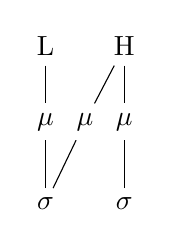
\begin{tikzpicture}
			\node (t1) at (1,1) {L};
			\node (t2) at (2,1) {H};
			
			\node[anchor=base] (c1) at (1,0) {$\mu$};
			\node[anchor=base] (c2) at (1.5,0) {$\mu$};
			\node[anchor=base] (c3) at (2,0) {$\mu$};
			
			\node (s1) at (1,-1) {$\sigma$};
			\node (s2) at (2,-1) {$\sigma$};
			
			\draw (t1) -- (c1);
			\draw (t2) -- (c2);
			\draw (t2) -- (c3);
			\draw (s1) -- (c1);
			\draw (s1) -- (c2);
			\draw (s2) -- (c3);            
		\end{tikzpicture} \vspace{2em}
		\subcaption{AR}
		
		\label{fig.model.AR1}
	\end{minipage}
	\hfill
	% Graph Representation
	\begin{minipage}[b]{0.4\textwidth}
		\centering
		\begin{tikzpicture}[scale=0.5]
			\node[state] (t1) at (0,6) {1\textsubscript{L}};
			\node[state] (t2) at (6,6) {2\textsubscript{H}};
			
			\node[state] (c1) at (0,3) {3\textsubscript{$\mu$}};
			\node[state] (c2) at (3,3) {4\textsubscript{$\mu$}};
			\node[state] (c3) at (6,3) {5\textsubscript{$\mu$}};
			
			\node[state] (s1) at (0,0) {6\textsubscript{$\sigma$}};
			\node[state] (s2) at (6,0) {7\textsubscript{$\sigma$}};
			
			\draw (t1) -- node[midway, left]   {$\alpha$} (c1) -- node[midway, left]
			{$\alpha$}(s1);
			\draw (t2) -- node[midway, left] {$\alpha$} (c2) -- node[midway, left]
			{$\alpha$}(s1);
			\draw (t2) -- node[midway, right] {$\alpha$} (c3) -- node[midway, right]
			{$\alpha$}(s2);
			
			
			\draw (t1) -- node[midway, above]  {$\lhd$} (t2);
			\draw (c1) -- node[midway, above]  {$\lhd$}(c2);
			\draw (c2) -- node[midway, above]  {$\lhd$}(c3);
			\draw (s1) -- node[midway, above]  {$\lhd$}(s2);
		\end{tikzpicture}
		\subcaption{Graph}
		\label{fig.model.AR2}
	\end{minipage}
	\hfill
	% Model Representation
	\begin{minipage}[b]{0.3\textwidth}
		\small
		\centering
		\begin{align*}
			%            M &= \langle D|  H, L, \mu, \sigma, \lhd, \alpha \rangle \\
			D &= \{1, 2, 3, 4, 5, 6, 7\} \\
			L &= \{1\}\\
			H &= \{2\}\\
			\mu &= \{3, 4, 5\}\\
			\sigma &= \{6, 7\} \\
			\lhd &= \{\, \langle 1,2 \rangle, \langle 3,4 \rangle, \langle 4,5 \rangle,
			\langle 6,7 \rangle\} \\
		\alpha &= \left\{
		\begin{aligned}
			&(1,3),(2,4),(2,5),\\
			&(3,6),(4,6),(5,7)
		\end{aligned}
		\right\}
		\end{align*}
		\subcaption{Model}
		\label{fig.model.AR3}
	\end{minipage}
	
	
	\caption{Three representations of a disyllabic LH.H}
	\label{fig.model.AR}
\end{figure}

A graph consists of a set of vertices $V$ and edges $E$.  
As shown in Figure~\ref{fig.model.AR3}, the graph consists
of seven \textit{labelled nodes} which are circles numbered with $\{1, 2,\dots,7\}$, 
representing linguistic units, each labelled with its corresponding properties, such
as $L$, $H$, $\sigma$, or $\mu$. 
The lines connecting elements are referred to as \textit{edges}, which 
may be either \textit{directed} or \textit{undirected}. For clarity, 
we distinguish two types of connections: \textit{association relations}, 
denoted by $\alpha$, refer to the undirected edges across tiers; 
%(e.g., between tones and moras, or between moras and syllables), 
and successor relations, denoted by $\lhd$, represent ordered relationships within a single tier. 
All the successor connections in the current example are given by
\( \lhd = \{\langle 1,2 \rangle,\ \langle 3,4 \rangle,\ \langle 4,5
\rangle,\ \langle 6,7 \rangle \}.\) The association relations, on the
other hand, are expressed as a set of unordered pairs:
\(\alpha = \{ (1,3),\ (2,4),\ (2,5),\ (3,6),\ (4,6),\ (5,7) \}.\)
Together, the tuple $\langle H, L, \mu, \sigma, \lhd, \alpha \rangle$
constitutes the \textit{signature} of this model-theoretic representation
of an AR.

In addition to representing model-theoretic relational structures 
with graphs, one can use \textit{adjacency matrices}
\citep{west2001introduction,CLRS2022}, which use binary values to
denote whether there is an edge between two nodes. Two nodes, $v$ and
$w$, are considered \textit{adjacent} if there is an edge connecting
them. If $G$ is a graph with $n$ nodes %,labelled $\{1, 2, \ldots, n\}$,
then its adjacency matrix $A$ is an $n \times n$ matrix. If $i$ and 
$j$ are connected, the entry $(i, j)$ has the value of 1; otherwise it is
0. 
Using this method, an AR with $t$ tones, $m$ moras, and $s$ 
syllables can be encoded as a $t \times m$ tone-mora matrix and 
a $m \times s$ mora-syllable matrix, with successor relations 
implicit in the indexing. For instance, Table~\ref{tab.matrices} provides an alternative
representation of the same AR in Figure~\ref{fig.model.AR}.
In the tone-mora matrix, the header row reflects the tonal sequence
$LH$, and the index column reflects the mora sequence. Since the L tone is
associated with the first mora $\mu_1$, and the H tone is associated with
both $\mu_2$ and $\mu_3$, the corresponding cells
$(L, \mu_1), (H, \mu_2), (H, \mu_3)$ are marked with 1, and the others
with 0 which indicates no connection between them.\footnote{For
	convenience, we refer to each cell by the labels of the nodes. Node
	indices will be omitted from here on. For example, we may refer to $(1,3)$
	and $(2,4)$ with $(L,\mu_1)$ and $(H, \mu_2)$, respectively. However, 
	these are the labels of the nodes rather than the nodes 
	themselves.}  If we examine the matrix by columns, one can infer that
the L tone occupies the first mora, while the H tone occupies the
remaining two.  Likewise, in the mora syllable matrix, since
$\sigma_1$ is associated with $\mu_1$ and $\mu_2$, and $\sigma_2$ with
$\mu_3$, the corresponding cells are marked with 1. If we examine this
matrix by rows, it can be seen that $\sigma_1$ is heavy while
$\sigma_2$ is light. Hereafter, we refer to the rows and columns in
the tone-mora matrix as the mora rows and tone columns respectively;
and to the rows and columns in the mora-syllable matrix as the
syllable rows and mora columns respectively.
\begin{table}[ht]
\centering 
	\begin{tabular}{cc}
	\centering
	\begin{tabular}{c|cc}
			& L & H \\
			\hline
			$\mu_1$ & 1 & 0 \\
			$\mu_2$ & 0 & 1 \\
			$\mu_3$ & 0 & 1 \\
	\end{tabular} \vspace{1em}
		&
	\begin{tabular}{c|ccc}
			& $\mu_1$ & $\mu_2$ & $\mu_3$ \\ \hline
			$\sigma_1$ & 1     & 1     & 0     \\
			$\sigma_2$ & 0     & 0     & 1
	\end{tabular}
	\end{tabular}
	\caption{Adjacency matrices: tone–mora matrix (left) and mora–syllable matrix (right)}
	
	\label{tab.matrices}
\end{table}

These AR adjacency matrices capture precisely the same information as
the graphs and model-theoretic structures. If we replace the header
row and index column with the node numbers used in the graph model
signature, and replace the 1s with the indices of row and column, we
obtain the table filled as in Table~\ref{tab.index}. As can be
seen, these pairs are identical to the information encoded in
Figure~\ref{tab.matrices}.

\begin{table}[ht]
	\centering
	\begin{tabular}{cc}
		$\begin{array}{c|c@{}c@{}c}
			& 1 & \lhd & 2 \\
			\hline
			3 & (1,3)  && 0 \\
			\lhd & && \\
			4 & 0 & & (2,4) \\
			\lhd & && \\
			5 & 0 & & (2,5) \\
		\end{array}$ \hspace{1em} &
		$\begin{array}{c|c@{}c@{}c@{}c@{}c}
			& 3 & \lhd & 4 & \lhd & 5 \\
			\hline
			6           & (3,6) &         & (4,6) &         &   	\\
			\lhd  &       &         &       &         &   	\\
			7           &       &         &       &         & (5,7) \\
		\end{array}$
	\end{tabular}
\caption{Equivalent node-indexed encodings of the adjacency matrices in Table~\ref{tab.matrices}, where $\lhd$ and $\alpha$ are the successor and association predicates of the model signature.}
	\label{tab.index}
\end{table}

Furthermore, certain patterns can be easily identified by inspecting the
matrices. For example, a series of contiguous 1s may indicate tone 
spreading over multiple moras if observed in the tone column, or a mora 
shared by multiple tones if seen in the mora row. 
Two 1s positioned diagonally suggest a one-to-one mapping.
The associations $(L,\mu_1)$ and $(H,\mu_2)$
in the tone-mora matrix in Table \ref{tab.matrices}
present an example of this.
Some particular or ill-formed patterns can also be 
readily detected, which will be discussed in Section~\ref{sec:bufiaar}.


\subsection{Structure Containment}
%
An important concept when considering model-theoretic relational
structures, either strings, sequences of feature bundles, or ARs, is
\textit{containment}. Intuitively, containment refers to the situation
when one structure includes another structure inside of it. We
formalise this notion using two related definitions, following
\citet{chandleeBufia2019}: \textit{restriction}
(Definition~\ref{def.res}) and \textit{containment}
(Definition~\ref{def.contain}). Readers are referred to
\citet{rogers.lambert2019mol} for an alternative formulation. In the
definitions below, it is assumed the structures A and B have the same
signature $\langle R_1, \ldots R_n \rangle$.

\begin{definition}
	\label{def.res}
	\textit{ $A= \langle D^A; R^A_1, \ldots, R^A_n \rangle$ is a \emph{restriction}
		of $B
		= \langle D^B; R^B_1, \ldots, R^B_n \rangle$ iff $D^A \subseteq D^B$ and for
		each $m$-ary relation $R^A_i$, we have $R^A_i = \{(x_1, \ldots, x_m) \in R^B_i \mid x_1, \ldots, x_m \in D^A\}$. }
\end{definition}

\begin{definition}
	\label{def.contain}
	\textit{Structure $A$ is \emph{contained} in structure $B$
		($A \sqsubseteq B$) if there exists a restriction of $B$, denoted
		$B'$, and there exists a function $h:A \rightarrow B'$ such that for
		each $m$-ary relation $R_i$ in the model signature:
		\(R_i(a_1, \ldots, a_m) \in A \implies R(h(a_1), \ldots, h(a_m)) \in
		B'.\)}
\end{definition}

These definitions mean that $A$ is \textit{contained} in $B$ whenever
there exists a subpart of $B$ onto which \(A\) projects via a function
\(h\), and furthermore, that the relations that hold among elements of
\(A\) hold among their corresponding elements in \(B\). For instance,
the AR in Figure~\ref{fig.restriction:a} is contained in the AR
in Figure~\ref{fig.restriction:b} because the dotted region in
\ref{fig.restriction:b} preserves all internal relations of
%:
\ref{fig.restriction:a}, despite the differences in the
indexing. In particular, $\mu_1, \mu_2, \sigma_1$ in
\ref{fig.restriction:a} project to $\mu_2, \mu_3, \sigma_2$ in
\ref{fig.restriction:b}, respectively.


\begin{figure}[h]
	\centering
	\begin{minipage}[t]{0.32\textwidth}
		
		
		\centering
		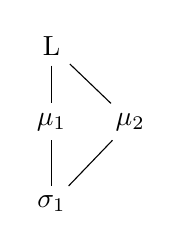
\begin{tikzpicture}
			\node (t2) at (1,1) {L};
			
			\node[anchor=base] (c1) at (1,0) {$\mu_1$};
			\node[anchor=base] (c2) at (2,0) {$\mu_2$};
			
			\node (s2) at (1,-1) {$\sigma_1$};
			\draw (t2) -- (c1) -- (s2);
			\draw (t2) -- (c2) -- (s2);
			
		\end{tikzpicture} 
		\subcaption{Heavy L syllable}
		\label{fig.restriction:a}
	\end{minipage}	
	\begin{minipage}[t]{0.32\textwidth}
		\begin{tikzpicture}
			\node (t1) at (1,1) {H};
			\node (t2) at (2,1) {L};
			\node (t3) at (3,1) {H};
			
			\node[anchor=base] (c1) at (1,0) {$\mu_1$};
			\node[thick, anchor=base] (c2) at (2,0) {$\mu_2$};
			\node[thick, anchor=base] (c3) at (3,0) {$\mu_3$};
			
			\node (s1) at (1,-1) {$\sigma_1$};			
			\node (s2) at (2,-1)  {$\sigma_2$};
			\draw (t1) -- (c1) -- (s1);
			\draw (t2) -- (c1) -- (s1);
			\draw (t2) -- (c3) --(s2);
			\draw  (t2) -- (c2) -- (s2);
			\draw  (t3) -- (c3);
			\draw[dotted, thick]
			($(t2)+(-0.3,0.3)$) --
			($(t2)+(0.2,0.3)$) --
			($(c3)+(0.3,0.2)$) --
			($(c3)+ (0.3,0.2) + (0,-0.45)$) --
			($(s2)+(0.2,-0.3)$) --
			($(s2)+(-0.3,-0.3)$) --
			cycle;
			
			
		\end{tikzpicture} 
		\subcaption{AR containing a heavy L}
		\label{fig.restriction:b}
	\end{minipage}
	\caption{A heavy L-toned syllable and a structure in which it is contained}
	\label{fig.restriction}
\end{figure}


The containment relation is particularly important because it provides
a natural \textit{ordering} over the space of possible structures. The
ordering is not total, like a linear order; it is a \textit{partial}
ordering. In such a partially-ordered space, some structures are
comparable in terms of containment, but not necessarily all of them
are. \citet{chandleeBufia2019} provides some additional terminology:
if one structure \(A\) is contained in another structure \(B\), then
structure \(A\) is a \textit{subfactor} of structure \(B\), whereas
\(B\) is a \textit{superfactor} of \(A\). They prefer these terms to
substructures and superstructures, which have different
technical meanings in model theory.

To illustrate, Figure~\ref{fig.hasse.str} displays a
non-exhaustive portion of the partial ordering of possible strings
over the alphabet $\Sigma = \{a,b\}$. At the bottom of the ordering is
the empty string $\epsilon$, with more complex strings appearing
higher in the ordering.  Whenever two elements are connected by a
line, it means that the higher element contains the lower element. For
example, no line relates the \(a\) to \(b\), because neither contains
the other.  However, a line is drawn from \(a\) to \(aa, ab\) and
\(ba\), because \(a\) is contained in each of these structures. As
defined above, \(aa, ab, ba\) and \(aaa\), and any other strings that
contain \(a\) are superfactors of \(a\); correspondingly, \(a\) is a
subfactor of each of these strings.

There can be many layers between a superfactor and one of its 
subfactors. When there are no structures ordered 
between a superfactor and one of its subfactors, the 
superfactor is called a \textit{next superfactor}. 
In this sense, among all superfactors of \(a\) such as 
\(\{aa, ab, ba, aaa, aab, \cdots\}\), only those superfactors that 
are exactly one level above are next superfactors of \(a\), 
namely \(\{aa, ab, ba\}\).

\begin{figure}
	\centering
	\begin{tikzpicture}[
		every node/.style={inner sep=1pt, font=\small\itshape},
		edge/.style={},
		]
		\matrix (m) [matrix of nodes,
		row sep=6mm,
		column sep=10mm,
		nodes={anchor=center},
		]{
			\node (aaa) {aaa}; &\node (llb1) {...};&   \node (llb2) {...}; & \node (llb3) {...};&\node (llb4) {...};&\node (llb5) {...};&    \node (bbb) {bbb}; \\
			&\node (aa) {aa}; & \node (ab) {ab}; && \node (ba) {ba}; & \node (bb) {bb}; \\
			&& \node (a) {a}; & & \node (b) {b}; &  \\
			&&& \node (z) {$\epsilon$}; && \\};
		
		\draw[edge] (z) -- (a);
		
		\draw[edge] (z) -- (b);
		
		\draw[edge] (a) -- (aa) -- (aaa);
		\draw[edge] (a) -- (ab);
		\draw[edge] (a) -- (ba);
		
		\draw[edge] (b) -- (bb) -- (bbb);
		\draw[edge] (b) -- (ab);
		\draw[edge] (b) -- (ba);
		\draw[edge, dotted] (aa) -- ++(0,1.5em);
		%	\draw[edge, dotted] (aa) -- ++(1,1.5em);
		\draw[edge, dotted] (ab) -- ++(0,1.5em);
		%	\draw[edge, dotted] (ab) -- ++(1,1.5em);	
		%	\draw[edge, dotted] (bb) -- ++(-1,1.5em);	
		\draw[edge, dotted] (ba) -- ++(0,1.5em);
		\draw[edge, dotted] (bb) -- ++(0,1.5em);
	\end{tikzpicture}
	\caption{Strings over $\Sigma = \{a,b\}$ ordered by the containment relation (non-exhaustive)}
	\label{fig.hasse.str}
\end{figure}%



\subsection{BUFIA}\label{sec:prelim.bufia}

Recall that given a set of positive examples, BUFIA returns a grammar just like
the ones considered by \citet{jardine2017LocalNature}: a conjunction
of negative literals: $\lnot C_1 \land \lnot C_2 \land \ldots \land \lnot C_n$.
BUFIA begins its search of the possible structure space with the most
general structure (the empty structure) and progresses to more
specific ones. In other words, it proceeds from the bottom of the
inverted pyramid upwards. In this process, two functions are central 
to BUFIA: \textsc{Contain} and \textsc{NextSupFact}. For each 
candidate structure \(S\), BUFIA applies the
\textsc{Contain} function to check whether it is attested
in the positive data. If it is, BUFIA concludes it is not a bona-fide
constraint, discards it, and uses \textsc{NextSupFact} to generate a
set of next superfactors to continue the search. If, on the other
hand, \(S\) is absent from the positive data, it is added to the
grammar as a constraint. For structures that are labelled as constraints,
BUFIA does not apply \textsc{NextSupFact}. Consequently, all structures/possible 
constraints that contain it are pruned from the remaining search. The learning 
process continues until a stopping condition is met, which in this work is a
predetermined upper bound on the size of the constraints.

Using the same example from Figure~\ref{fig.hasse.str}, suppose
the language forbids adjacent \(b\)s, formalised as a constraint
\(^*bb\), which excludes strings \(\{bb, bba, bbb, abb,
\cdots\}\). For concreteness, assume a data set \(D = 
\{aba, baabaa\}\).  BUFIA begins from the most general hypothesis:
applies \textsc{Contain} to check whether the empty string $\epsilon$
is attested in the positive data.  Since $\epsilon$ is contained in
every string trivially, \textsc{Contain} returns true, and BUFIA does
not add $\epsilon$ as a constraint. Then, BUFIA applies
\textsc{NextSupFact} to generate the next superfactors of $\epsilon$,
which are the two singletons \(a\) and \(b\). In a breadth-first
order, BUFIA checks whether \(a\) and \(b\) are contained in the
positive data.  In the same fashion, the \textsc{Contain} function
confirms both strings are attested as substrings of \(D\), discards
them, and then generates their superfactors for later checking. When
BUFIA reaches \(bb\), \textsc{Contain} returns false because
\(bb\) is not contained in any datum in the data set (neither \(aba\) nor 
\(baabaa\) contains \(bb\)). BUFIA therefore adds
\(^*bb\) to the grammar and skips generating any superfactors of
\(bb\). The search then continues with the remaining candidates until
the stopping condition is met (e.g., the size of structures exceeds a
predefined size such as two).\footnote{An alternative stopping
  condition is to set a number of constraints. Both kinds of stopping
  conditions control the amount of generalisation. The longer the
  search is permitted, more constraints may be found, and amount of
  generalisation is reduced. Without any limits, it will overfit the
  data. However, when the search terminates sooner, generally fewer
  constraints will be found, and the grammar makes broader
  generalisations.}

\citet{chandleeBufia2019} prove that BUFIA returns a set of
constraints that (1) are consistent with the data (no constraint
returned by BUFIA is contained in any datum in the positive data); (2)
contain the most general constraints (obtains the simplest possible
constraints according to the order imposed by the containment
relation, e.g.  only \(^*bb\) is returned but not \(^*bba\), \(^*bbb\)
or others); and (3) generate the smallest set of structures consistent
with the data, among the other possible grammars that are
consistent with the data subject to the same conditions (generalises
conservatively).

One concern for BUFIA is its time complexity: BUFIA runs in exponential time in the worst 
case \citep{chandleeBufia2019}. However, as \citet{Swanson+2025} 
point out, data sparsity is highly advantageous for learning since 
the hypothesis space is thus pruned more efficiently.

Another concern raised by the reviewers is that, in its
present form, BUFIA is fragile with respect to noise. For example, if
there is a single data point violating a constraint \(C\) in the
data (a ``noisy intrusion''), then \(C\) will not be included in the
output grammar, even if \(C\) is an otherwise valid
generalisation. It is important to put this current limitation in
context. First, even in the absence of noise, it is currently unknown
how to learn constraints expressed with ARs. From the viewpoint of
scientific practice, it makes sense to address an easier problem
before addressing a harder problem. Second, BUFIA can be adapted to
handle noise in different kinds of ways. Prior literature suggests
multiple strategies for handling noisy intrusions, exceptions, and
sparse data \citep{angluin88, Yang2016, Wu-Heinz-2023-SELDNI,
  Kaelbling+2023-RILIPD, Dai2025}. Considering versions of BUFIA that
are robust to all kinds of noise is a valuable direction for future
research. Third, it is worth pointing out that the mere use of
statistical methods for learning does not automatically make learners
robust to noise \citep{Angluin88b}. In other words, noisy data is an
issue, and one that can be studied separately from the fundamental
issue of successful generalisation. See \citet{Heinz2009} for
additional discussion on factoring learning problems.

\section{Learning over Autosegmental Representations} \label{sec:bufiaar}

This section introduces the BUFIA-AR in Section~\ref{sec:bufiaar.algo}.
Sections~\ref{sec:bufiaar.nextar} and \ref{sec:bufiaar.arcontain}, 
address how its two core functions, \textsc{NextSupFact} and 
\textsc{Contain}, are realised specifically for ARs.  Those sections will also demonstrate that the
use of adjacency matrices simplifies the computational implementation,
making it more straightforward and interpretable. Our goal is to walk
through each piece step by step, as they are essential for (i)
understanding the logical reasoning behind tonotactic learning over
ARs, (ii) properly interpreting the results that follow, and (iii)
replicating our study or adapting BUFIA-AR for other AR-like structures in future work.

\subsection{BUFIA-AR} \label{sec:bufiaar.algo}

BUFIA-AR instantiates BUFIA with ARs, and the \textsc{Contain} and
\textsc{NextSupFact} functions operate in the same manner as in
Section~\ref{sec:prelim.bufia} but only differ in representations.  In
the case of BUFIA-AR, the stopping condition is defined as
predetermined upper bounds on the numbers of tones, moras, and
syllables. These steps are formalised in Algorithm \ref{alg.bufia},
and are discussed in more detail below.  

\begin{algorithm}
	\caption{\textsc{Bottom-Up Factorial Inference Algorithm over Autosegmental Representations}}
	\label{alg.bufia}
	\begin{algorithmic}[1]
		\Require Positive data $D$, initial empty AR $ar_0$, maximum tier limits $t, m, s$
		\Ensure Set of learned generalisations $G$
		
		\State $Q \gets {ar_0}$ %\Comment{initialized with empty AR}
		\State $G \gets \emptyset$ %\Comment{Learned constraints}
		\State $V \gets \emptyset$ %\Comment{Visited structures}
		
		\While{$Q \neq \emptyset$}
		\State $ar \gets Q.\textsc{dequeue}()$ \label{dequeue}
		\If{$ar \notin V$}
		\State $V \gets V \cup \{ar\}$
		
		\If{$\exists x \in D \text{ s.t. } ar \sqsubseteq x$}
		%\Comment{$ar$ is attested in $D$}
		\State $\mathcal{A} \gets \textsc{NextSupFact}(ar)$
		%\Comment{Generate immediate superfactors of $ar$}
		
		\State $\mathcal{A}' \gets \{ ar' \in \mathcal{A} \mid$
  		$\text{size}(ar') \le (t, m, s)$
		$\land\ \nexists g \in G \text{ s.t. } g \sqsubseteq ar'$
		%\Comment{Filter oversized or illegal $ar'$}
		
		\State $Q.\textsc{enqueue}(\mathcal{A}')$ \label{enqueue}

		\Else
		%\Comment{$ar$ is unattested in $D$}
		\State $G \gets G \cup \{ar\}$
		%\Comment{Add $ar$ to grammar}
		\EndIf
		\EndIf
		\EndWhile
	
		\State \Return $G$
	\end{algorithmic}
\end{algorithm}


BUFIA-AR initially requires three inputs: a finite set of positive data
over ARs $D$, an initial empty AR \(ar_0\), and a set of maximum constraint 
limits \(t, m, s \in\mathbb{N}\). The positive data \( D \) contains 
a finite set of well-formed ARs. The positive integers \(t, m, s\) 
limit the numbers of tones, moras, and syllables of an AR considered by BUFIA-AR. 
Additionally, BUFIA-AR initialises two empty sets: \( G \), representing the 
grammar which is empty at first and will be returned with constraints 
discovered by the algorithm once the learning is complete; and a set \( 
V \) which stores checked ARs to avoid revisiting
superfactors that have already been examined.

A queue \(Q\) is used to store structures to be checked 
by BUFIA-AR, following a standard breadth-first search 
method. As shown in Line~\ref{dequeue} and \ref{enqueue},
there are two operations related to \(Q\): \textsc{dequeue} and
\textsc{enqueue}: the former takes an AR structure \(ar\) out of the queue
for checking against the data, and the latter adds the next structure
into \(Q\), making it available for the learner to evaluate later in a breadth-first
manner.

BUFIA-AR is called with the initial structure \( ar_0 \) set to the most
generalised and least complex structure, the empty structure. The
\textsc{Contain} function takes the current structure as an argument
and checks whether it is a subfactor of the data. If so, the
\textsc{NextSupFact} function generates its next superfactors
which must also satisfy the following conditions: the tone,
mora, and syllable of an AR do not exceed \(t, m, s\),
have not yet been visited, and do not contain any structures
already forbidden by the grammar. The eligible superfactors will be
``enqueued'' for later checking. If the current structure is
absent from the dataset---that is, it is not a
subfactor of any data point---then it is added to $G$. This process
repeats until the size of the structure exceeds the predetermined
threshold \(t, m, s\).

As mentioned, function \textsc{Contain} and \textsc{NextSupFact} are
crucial in the implementation of BUFIA-AR. In the following sections,
we will first introduce how to expand a given AR to get its next
superfactors (Section \ref{sec:bufiaar.nextar}). Then we explain how to check
whether one AR is contained within another (Section
\ref{sec:bufiaar.arcontain}).

\subsection{How to Expand Autosegmental Representations}
\label{sec:bufiaar.nextar}

Here we explain how we compute the next superfactors of an AR. This
can be achieved by adding new units to tiers or by adding associations
between tiers. In a general graph-theoretic setting, any addition at
any position would in principle be allowed when constructing a
supergraph. However, for ARs, two principles must be taken into
account: linguistic meaningfulness and computational efficiency.

By linguistic meaningfulness, we require that the resulting graphs be
linguistically interpretable and obey basic universal constraints on
phonological representations. For example, expansions that result in
inconsistent tier projections, such as adding a mora to the tonal
melody tier, or expansions resulting line crossing, will be excluded. Examples of linguistically
invalid expansions are shown in Figure~\ref{fig.invalid.AR}
with dotted lines indicating impossible associations.
\begin{figure}[h]
	\centering
		\begin{tikzpicture}
			\node (s1) at (0,0) {$\sigma_1$};
			\node (m1) at (0,1) {$\mu_1$};
			\node (t1) at (0,2) {H};
			\node (t2) at (1,2) {$\mu_2$};
			\draw [-] (t1) to (m1) to (s1);
			\draw [-, thick, dotted] (t1) -- (t2); %node[midway] {$\times$};
		\end{tikzpicture} \hfil
		\begin{tikzpicture} 
			\node (s1) at (0,0) {$\sigma_1$};
			\node (m1) at (0,1) {$\mu_1$};
			\node (t1) at (0,2) {H};
			\node (m2) at (1,1) {L};
			\draw [-] (t1) to (m1) to (s1);
			\draw [-,thick, dotted] (m1) -- (m2); %node[midway] {$\times$};
		\end{tikzpicture} \hfil
		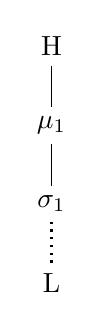
\begin{tikzpicture} 
			\node (s1) at (0,0) {$\sigma_1$};
			\node (m1) at (0,1) {$\mu_1$};
			\node (t1) at (0,2) {H};
			\node (m2) at (0,-1) {L};
			\draw [-] (t1) to (m1) to (s1);
			\draw [-,thick, dotted] (s1) -- (m2); %node[midway] {$\times$};
		\end{tikzpicture}\hfil
		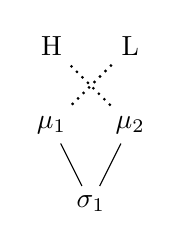
\begin{tikzpicture} 
			\node (s1) at (0.5,0) {$\sigma_1$};
			\node (m1) at (0,1) {$\mu_1$};
			\node (m2) at (1,1) {$\mu_2$};
			\node (t1) at (0,2) {H};
			\node (t2) at (1,2) {L};
			\draw [-,thick, dotted] (t1) to (m2);
			\draw [-,thick, dotted] (t2) to (m1);
			\draw [-] (s1) to (m2);
			\draw [-] (s1) to (m1);
		\end{tikzpicture}
		
		\caption{Invalid AR Expansions}
	\label{fig.invalid.AR}
\end{figure}
By computational efficiency, we aim to obtain distinct graphs while
minimising redundant construction of identical structures. In many
cases, the same resulting AR can be obtained via multiple expansion
paths. For example, inserting a mora between two existing moras may
yield the same structure as appending a mora to the right edge of the
tier or prefixing one to the left edge. Such redundant derivations
incur unnecessary computational cost by repeating equivalent work, and
we therefore seek to avoid them.

\subsubsection{Adding Units}
Based on these considerations, we require that new elements be added 
only to their projected tiers and only append them to the right 
edge, consistent with the temporal relation. This yields three specific
Expansion Rules (ERs):
\begin{itemize}
	\item \textbf{ER1} Append a tone to the tone tier.
	\item \textbf{ER2} Append a mora to the mora tier.
	\item \textbf{ER3} Append a monomoraic syllable to the syllable tier.
\end{itemize}
ERs (1–3) specify how a new tone, mora, or syllable can be appended 
to the end of each tier, analogously to extending a string.
Figure~\ref{fig.newars} illustrates how the base AR in 
Figure~\ref{ar:base} can be expanded in three different ways: by 
adding a tone L (\ref{ar:sup1}); by adding a monomoraic syllable $\sigma_2$, 
which by default associates to a single mora $\mu_2$ (\ref{ar:sup2}); 
or by adding a mora to the rightmost syllable (\ref{ar:sup3}).

\begin{figure}[ht]
\setlength{\tabcolsep}{4pt}
	\centering
	% --- First subtable ---
	\begin{minipage}[t]{0.2\textwidth}
		\centering
		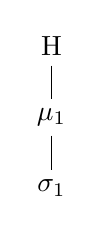
\begin{tikzpicture}[scale = 0.9] 
			\node (s1) at (0,0) {$\sigma_1$};
			\node (m1) at (0,1) {$\mu_1$};
			\node (t1) at (0,2) {H};
			\draw [-] (t1) to (m1) to (s1);
		\end{tikzpicture}
		
		\vspace{1em}
		
		\begin{tabular}{c|c}
				& \text{H} \\
				\hline
				$\mu_1$ & 1 \\
		\end{tabular}\vspace{2em}


		\begin{tabular}{c|c}
				& $\mu_1$ \\
				\hline
				$\sigma_1$ & 1 \\
		\end{tabular}
		\vspace{1.5em}
		\subcaption{Base AR}\label{ar:base}
	\end{minipage}
	\hfill
	% --- Second subtable ---
	\begin{minipage}[t]{0.2\textwidth}
		\centering
		\begin{tikzpicture}[scale = 0.9]
			\node (s1) at (0,0) {$\sigma_1$};
			\node (m1) at (0,1) {$\mu_1$};
			\node (t1) at (0,2) {H};
			\node (t2) at (1.2,2) {L};
			\draw [-] (t1) to (m1) to (s1);
			\draw [->, >=Latex, dotted,thick] (t1) to (t2);
		\end{tikzpicture}
		
		\vspace{1em}
		
		\begin{tabular}{c|cc}
				& H & L \\
				\hline
				$\mu_1$ & 1 & \textbf{0}\\
		\end{tabular}\vspace{2em}


		\begin{tabular}{c|c}
				& $\mu_1$ \\
				\hline
				$\sigma_1$ & 1 \\
		\end{tabular}
		\vspace{1.5em}
		\subcaption{Add a tone}\label{ar:sup1}
	\end{minipage}	\hfill
	% --- Third subtable ---
	\begin{minipage}[t]{0.2\textwidth}
		\centering
		\begin{tikzpicture}[scale = 0.9]
			\node (s1) at (0,0) {$\sigma_1$};
			\node (s2) at (1.2,0) {$\sigma_2$};
			\node (m1) at (0,1) {$\mu_1$};
			\node (t1) at (0,2) {H};
			\node (m2) at (1.2,1) {$\mu_2$};
			\draw [-] (t1) to (m1) to (s1);
			\draw [->,>=Latex, dotted,thick] (s1) to (s2);
			\draw [-] (m2) to (s2);
			\draw [->,>=Latex, dotted,thick] (m1) to (m2);
		\end{tikzpicture}
	
		\vspace{1.1em}
		
		\begin{tabular}{c|c}
			& \text{H} \\
			\hline
			$\mu_1$ & 1 \\
			$\mu_2$ & \textbf{0} \\
		\end{tabular}\vspace{1em}
		\begin{tabular}{c|cc}
			& $\mu_1$ & $\mu_2$ \\
			\hline
			$\sigma_1$ & 1 & 0\\
			$\sigma_2$ & 0 & \textbf{1}\\
		\end{tabular}
		\subcaption{Add a syllable}\label{ar:sup2}
	\end{minipage}	\hfill
	\begin{minipage}[t]{0.2\textwidth}
		\centering
		\begin{tikzpicture}[scale = 0.9]
			\node (s1) at (0,0) {$\sigma_1$};
			\node (m1) at (0,1) {$\mu_1$};
			\node (t1) at (0,2) {H};
			\node (m2) at (1.2,1) {$\mu_2$};
			\draw [-] (t1) to (m1) to (s1);
			\draw [-, dotted,thick] (m2) to (s1);
			\draw [->,>=Latex, dotted, thick] (m1) to (m2);
		\end{tikzpicture}
		
		\vspace{1.1em}
		
		\begin{tabular}{c|c}
			& \text{H} \\
			\hline
			$\mu_1$ & 1 \\
			$\mu_2$ & \textbf{0} \\
		\end{tabular}\vspace{1em}
		\begin{tabular}{c|cc}
			& $\mu_1$ & $\mu_2$ \\
			\hline
			$\sigma_1$ & 1 & \textbf{1}\\
		\end{tabular}
		\vspace{1em}
		\subcaption{Add a mora}\label{ar:sup3}
	\end{minipage}
	\hfill
	% --- Fourth subtable ---
	\caption{Base AR and its superfactors by adding a new tone,
		syllable, and mora}
	\label{fig.newars}
\end{figure}


One might wonder how ER1 relates to the Obligatory Contour Principle
(OCP). There is cross-linguistic evidence for pressures to avoid
sequences of identical tones, although whether the OCP should be a
universal rule has been debated \citep{goldsmith1976autosegmental,
	meyers1997ocp}. 
	
Our Hausa case study enforces the OCP by 
appending a tone that differs from the final 
tone in the current AR. There are two reasons for this practice. First, there is no clear evidence 
that argues against the OCP in Hausa; second, enforcing the OCP also 
helps reducing the search space by restricting tonal sequences. 
Nonetheless, relaxing this restriction is possible and is left 
for future research.


\subsubsection{Adding Association Lines}
Besides adding units, an AR can also be changed by modifying an 
association line and leaving the number of the segments or features 
unchanged. This ability to manipulate associations independently 
of segments forms the core mechanism of autosegmental theory. 
Concerning the association lines, \citet{goldsmith1976autosegmental} 
proposes a set of well-formedness conditions (WFCs) as a guidance 
of how association lines may be added or deleted. These conditions 
require association changes to be minimal while maximising satisfaction 
of basic representational requirements.

\begin{enumerate}
	\setlength\itemsep{0em}
	\setlength\parskip{0em}
	\item All vowels are associated with at least one tone.
	\item All tones are associated with at least one vowel.
	\item Association lines do not cross (No-Crossing Constraint, NCC)
\end{enumerate}

From a computational perspective, unrestricted growth of association lines is costly, as it allows arbitrary connections between any two nodes.
The NCC plays a crucial role in reducing this complexity by limiting the 
set of admissible association lines. There have been several works 
providing formal definitions of the WFCs \citep{goldsmith1976autosegmental, 
	coleman1991no, jardine2015concatenation, jardine2017LocalNature}. 
Based on these, the NCC rule can be formalised as following. Letting \(\alpha\) be the set of existing associations, a new association \((i,j)\) is valid if 
and only if there does not exist an association \((i',j') \in \alpha\) such 
that \( (i' > i \wedge j' < j) \;\vee\; (i' < i \wedge j' > j)\). 

At the same time, to further avoid adding association lines which give
rise to identical graphs, we impose an additional constraint for
computational efficiency: an association line may be added only to the
the first unassociated unit. In other words, a fully-specified AR (all tones, moras, syllables are already associated with at least one element), will not add new association lines. If an AR contains more than one unassociated unit,
the new association must be formed to the first available unassociated
unit. This is to satisfy WFC 1 and 2. Finally, from a linguistic
perspective, we assume that the association lines between moras and
syllables are pre-specified. Consequently, new association lines are
formed only between moras and tones. This yields the ER4:\\

\noindent \textbf{ER4} Add an association line between tone and mora, subject to the following conditions:
	\begin{enumerate}[label = \alph*.]
		\setlength\itemsep{0em}
		\setlength\parskip{0em}
		\setlength{\parindent}{1em}
		\item do not violate the No-Crossing Constraint;
		\item involve at least one unassociated unit; and
		\item be formed adjacent to the final mora--tone association.\label{er4}
	\end{enumerate}

The final tone-mora association in an AR can be expressed 
mathematically as in Definition~\ref{def.finaltonemora}.

\begin{definition}
	\label{def.finaltonemora}
	\textit{An edge $(t,m)$ in the tone--mora matrix is defined as the final tone--mora association if $t \in H \cup L$, $m \in 
		\mu$, and $(t,m) \in \alpha$, and there exists no edge $(t',m') \in
		\alpha$ such that $t' > t$ or $m' > m$.}
\end{definition} 

Once the final tone-mora association is identified at $(t, m)$, there are 
three options, as listed in Definition~\ref{def.newassoc}, to form an association line $(t', m')$ while adhering to ER4:


\begin{definition}
	\textit{
		Given the final tone--mora association $(t,m)$, a new edge $(t',m')$
		adjacent to $(t,m)$ can be formed in three ways:}
	\begin{enumerate}[label = \alph*.]
		\setlength\itemsep{0em} \setlength\parskip{0em}
		\item $(t', m') = (t{+}1,\, m)$ \qquad\, \textit{if} $\, t{+}1 \in D$  
		\item $(t', m') = (t,\, m{+}1)$ \qquad\, \textit{if} $\, m{+}1 \in D$  
		\item $(t', m') = (t{+}1,\, m{+}1)$ \quad\, \textit{if} $ \, t{+}1,\, m{+}1 \in D$
	\end{enumerate}
	\label{def.newassoc}
\end{definition} 


For example, the AR in Figure~\ref{assoc0} contains an unassociated H tone 
and two unassociated moras, $\mu_3$ and $\mu_4$, as reflected by zeros in 
the tone--mora matrix. Taking the final association $(L,\mu_2)$ as the 
reference point, three new ARs can be formed by adding one adjacent 
association: (i) linking the unassociated tone to the nearest mora 
(Figure~\ref{new.assoc1}); (ii) linking an unassociated mora to the 
nearest tone (Figure~\ref{new.assoc2}); or (iii) directly linking an
unassociated tone and an unassociated mora (Figure~\ref{new.assoc3}).
\begin{figure}[ht]
\setlength{\tabcolsep}{4pt}
	\begin{minipage}{0.22\textwidth}
		\small
		\centering
		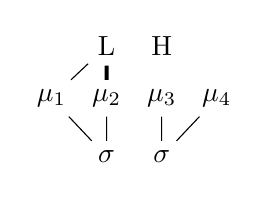
\begin{tikzpicture}[scale = 0.7]
			\node (t1) at (2,1) {L};
			\node (t2) at (3,1) {H};
			
			\node[anchor=base] (c1) at (1,0) {$\mu_1$};
			\node[anchor=base] (c2) at (2,0) {$\mu_2$};
			\node[anchor=base] (c3) at (3,0) {$\mu_3$};
			\node[anchor=base] (c4) at (4,0) {$\mu_4$};
			
			\node (s1) at (2,-1) {$\sigma$};
			\node (s2) at (3,-1) {$\sigma$};
			\draw (t1) -- (c1) -- (s1);
			\draw [line width = 0.5mm] (t1) -- (c2);
			\draw (c2) -- (s1);
			\draw (s2) -- (c4);
			\draw (s2) -- (c3);
		\end{tikzpicture}
		
		\vspace{0.3em}
		
		\begin{tabular}{c|cc}
			& L & H \\
			\hline
			$\mu_1$ & 1 & 0 \\
			$\mu_2$ & \cellcolor{gray!80}1 & 0\\
			$\mu_3$ & 0 & 0 \\
			$\mu_4$ & 0 & 0 
		\end{tabular}
		\subcaption{}
		\label{assoc0}
	\end{minipage}\hfill
	\begin{minipage}{0.22\textwidth}
		\small		
		\centering
		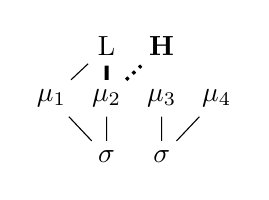
\begin{tikzpicture}[scale = 0.7]
			\node (t1) at (2,1) {L};
			\node (t2) at (3,1) {\textbf{H}};
			
			\node[anchor=base] (c1) at (1,0) {$\mu_1$};
			\node[anchor=base] (c2) at (2,0) {${\mu_2}$};
			\node[anchor=base] (c3) at (3,0) {$\mu_3$};
			\node[anchor=base] (c4) at (4,0) {$\mu_4$};
			\draw [line width = 0.5mm] (t1) -- (c2);		
			\node (s1) at (2,-1) {$\sigma$};
			\node (s2) at (3,-1) {$\sigma$};
			\draw (t1) -- (c1) -- (s1);
			\draw (c2) -- (s1);
			\draw (s2) -- (c4);
			\draw (s2) -- (c3);
			\draw [dotted, very thick] (c2) to (t2);
			
		\end{tikzpicture}
		
		\vspace{0.3em}
		
		\begin{tabular}{c|cc} 
			& L & H \\
			\hline
			$\mu_1$ & 1 & 0 \\
			$\mu_2$ & \cellcolor{gray!80}1 & \cellcolor{gray!30}1\\
			$\mu_3$ & 0 & 0 \\
			$\mu_4$ & 0 & 0 
		\end{tabular}
		\subcaption{}
		\label{new.assoc1}
	\end{minipage}
	\hfill
	% --- Second subtable ---
\begin{minipage}{0.23\textwidth}
			\small
		\centering
		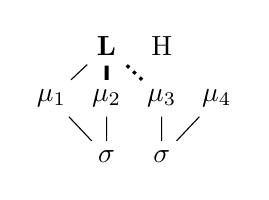
\begin{tikzpicture}[scale = 0.7]
			\node (t1) at (2,1) {\textbf{L}};
			\node (t2) at (3,1) {H};
			
			\node[anchor=base] (c1) at (1,0) {$\mu_1$};
			\node[anchor=base] (c2) at (2,0) {$\mu_2$};
			\node[anchor=base] (c3) at (3,0) {${\mu_3}$};
			\node[anchor=base] (c4) at (4,0) {$\mu_4$};
			
			\node (s1) at (2,-1) {$\sigma$};
			\node (s2) at (3,-1) {$\sigma$};
			\draw (t1) -- (c1) -- (s1);
			\draw (c2) -- (s1);
			\draw (s2) -- (c4);
			\draw (s2) -- (c3);
			\draw[dotted, very thick] (c3) to (t1);
			\draw [line width = 0.5mm] (t1) -- (c2);
		\end{tikzpicture}
		
		\begin{tabular}{c|cc}
			& L & H \\
			\hline
			$\mu_1$ & 1 & 0 \\
			$\mu_2$ & \cellcolor{gray!80}1 & 0 \\
			$\mu_3$ & \cellcolor{gray!30}1 & 0 \\
			$\mu_4$ & 0 & 0
		\end{tabular}
		\subcaption{}
		\label{new.assoc2}
	\end{minipage}
	\hfill
	% --- Third subtable ---
\begin{minipage}{0.23\textwidth}
			\small
		\centering
		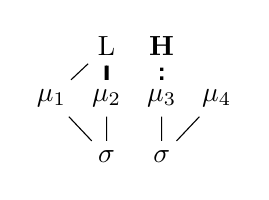
\begin{tikzpicture}[scale = 0.7]
			\node (t1) at (2,1) {L};
			\node (t2) at (3,1) {\textbf{H}};
			
			\node[anchor=base] (c1) at (1,0) {$\mu_1$};
			\node[anchor=base] (c2) at (2,0) {$\mu_2$};
			\node[anchor=base] (c3) at (3,0) {\textbf{$\mu_3$}};
			\node[anchor=base] (c4) at (4,0) {$\mu_4$};
			
			\node (s1) at (2,-1) {$\sigma$};
			\node (s2) at (3,-1) {$\sigma$};
			\draw (t1) -- (c1) -- (s1);
			\draw (t1) -- (c2) -- (s1);
			\draw (s2) -- (c4);
			\draw (s2) -- (c3);
			\draw [line width = 0.5mm] (t1) -- (c2);
			\draw[dotted, very thick] (c3) to (t2);
		\end{tikzpicture}
		
		\begin{tabular}{c|cc}
			& L & H \\
			\hline
			$\mu_1$ & 1 & 0 \\
			$\mu_2$ & \cellcolor{gray!80}1 & 0 \\
			$\mu_3$ & 0 & \cellcolor{gray!30}1\\
			$\mu_4$ & 0 & 0 
		\end{tabular}
		\subcaption{}
		\label{new.assoc3}
	\end{minipage}
	\caption{Three options to form new associations}
	\label{fig.newassoc}
\end{figure}


These operations offer several advantages both computationally and
linguistically. Computationally, we control the growth of the next
superfactors (by reducing the number of times a unique structure is
produced) without sacrificing expressiveness. We do not claim the
expansion rules are optimal, only that they outperform
naive approaches to superfactor generation.
Linguistically, these operations generate a full tonal inventory, 
including light, heavy, super-heavy syllables,
as well as simple and contour tones and tone-spreading patterns.

Recall from Section~\ref{sec:prelim} that factors stand in a 
containment relation, whereby superfactors contain subfactors. This 
relation yields a hypothesis space, illustrated in 
Figure~\ref{fig.AR.space}, in which lines (some shown as dotted for 
readability) connect a subfactor (lower-ranked) to its next superfactors 
(higher-ranked). If two factors are not connected by any path in this 
graph, they are incomparable, such as the unassociated H and the 
unassociated L.

\begin{figure}
	\centering
	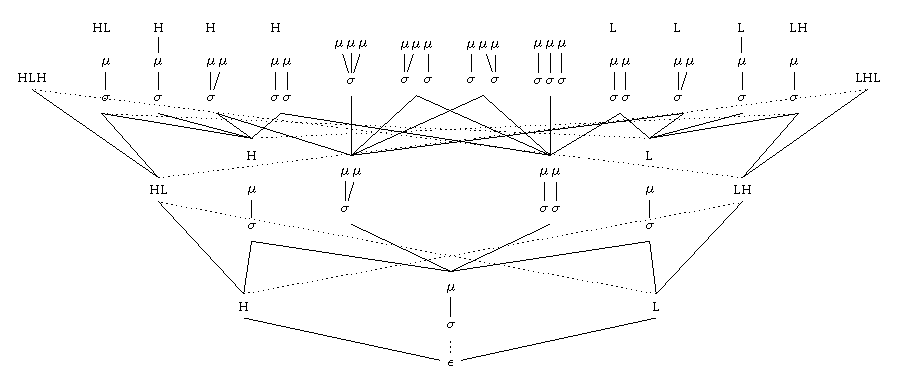
\includegraphics[scale=0.8]{figures/fig.space.pdf}
	\caption{A partially-ordered hypothesis space over ARs}
	\label{fig.AR.space}
\end{figure}

\subsubsection{Interim Summary}
\label{sec:bufiaar.summary}

To summarise, this subsection has presented a concrete method for
computing the next superfactors of a given AR. Four Expansion Rules
were defined: they expand the structure either by adding a unit on a
single tier or by introducing a new association.

We used adjacency matrices to represent the internal associations, and
stipulated some rules to reduce redundancy. Specific matrix patterns
were shown to diagnose ill-formed structures. For example,
Figure~\ref{fig.bad} illustrates three invalid ARs. An
anti-diagonal (from upper right to lower left) of 1s marks a
line-crossing violation, as in Figure~\ref{bad.assoc1}. A column or
row that is filled exclusively with zero indicates an unassociated tone or mora. Such zero-domination is
problematic when it occurs between two columns or rows that contain
associations, as this pattern indicates that an intervening unit has
been skipped, resulting in an improper association formed across it
(as in \ref{bad.assoc2} and \ref{bad.assoc3}) as they violate the
WFC 1 and 2.

\begin{figure}
	\centering	
	\setlength{\tabcolsep}{5pt}
	\begin{minipage}[t]{0.32\textwidth}
		\centering
		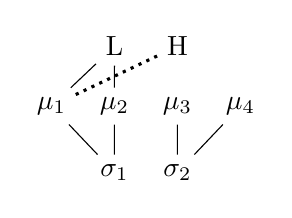
\begin{tikzpicture}[scale=0.8]
			\node (t1) at (2,1) {L};
			\node (t2) at (3,1) {H};
			\node[anchor=base] (c1) at (1,0) {$\mu_1$};
			\node[anchor=base] (c2) at (2,0) {$\mu_2$};
			\node[anchor=base] (c3) at (3,0) {$\mu_3$};
			\node[anchor=base] (c4) at (4,0) {$\mu_4$};
			\node (s1) at (2,-1) {$\sigma_1$};
			\node (s2) at (3,-1) {$\sigma_2$};
			\draw (t1) -- (c1) -- (s1);
			\draw (t1) -- (c2) -- (s1);
			\draw (s2) -- (c4);
			\draw (s2) -- (c3);
			\draw[dotted, line width=0.4mm] (c1) to (t2);
		\end{tikzpicture}
		
		\vspace{0.8em}
		
		\begin{tabular}{c|cc}
			& L & H \\
			\hline
			$\mu_1$ & 1 & \cellcolor{gray!30} 1 \\
			$\mu_2$ &\cellcolor{gray!30} 1& 0 \\
			$\mu_3$ & 0 & 0 \\
			$\mu_4$ & 0 & 0 \\
		\end{tabular}
		\subcaption{lines crossing}
		\label{bad.assoc1}
	\end{minipage}
	\hfill
	\begin{minipage}[t]{0.32\textwidth}
		\centering
		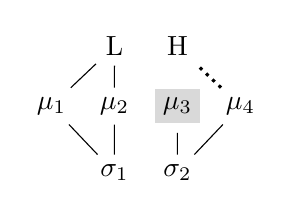
\begin{tikzpicture}[scale=0.8]
			\node (t1) at (2,1) {L};
			\node (t2) at (3,1) {H};
			\node[anchor=base] (c1) at (1,0) {$\mu_1$};
			\node[anchor=base] (c2) at (2,0) {$\mu_2$};
			\node[anchor=base] (c3) at (3,0) {\colorbox{gray!30}{$\mu_3$}};
			\node[anchor=base] (c4) at (4,0) {$\mu_4$};
			\node (s1) at (2,-1) {$\sigma_1$};
			\node (s2) at (3,-1) {$\sigma_2$};
			\draw (t1) -- (c1) -- (s1);
			\draw (t1) -- (c2) -- (s1);
			\draw (s2) -- (c4);
			\draw (s2) -- (c3);
			\draw[dotted, line width=0.4mm] (c4) to (t2);
		\end{tikzpicture}

		\vspace{0.8em}
		
		\begin{tabular}{c|cc}
			& L & H \\
			\hline
			$\mu_1$ & 1 & 0 \\
			$\mu_2$ & 1 & 0 \\
			\rowcolor{gray!30} $\mu_3$ & 0 & 0 \\
			$\mu_4$ & 0 & 1 \\
		\end{tabular}
		\subcaption{mora skipping}
		\label{bad.assoc2}
	\end{minipage}
	\hfill
	% --- Third subtable ---
	\begin{minipage}[t]{0.32\textwidth}
		\centering
		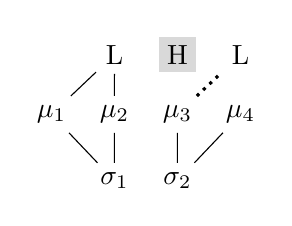
\begin{tikzpicture}[scale=0.8]
			\node (t1) at (2,1) {L};
			\node (t2) at (3,1) {\colorbox{gray!30}{H}};
			\node (t3) at (4,1) {L};
			\node[anchor=base] (c1) at (1,0) {$\mu_1$};
			\node[anchor=base] (c2) at (2,0) {$\mu_2$};
			\node[anchor=base] (c3) at (3,0) {$\mu_3$};
			\node[anchor=base] (c4) at (4,0) {$\mu_4$};
			\node (s1) at (2,-1) {$\sigma_1$};
			\node (s2) at (3,-1) {$\sigma_2$};
			\draw (t1) -- (c1) -- (s1);
			\draw (t1) -- (c2) -- (s1);
			\draw (s2) -- (c4);
			\draw (s2) -- (c3);
			\draw[dotted, line width=0.4mm] (c3) to (t3);
		\end{tikzpicture}
		
		\vspace{0.8em}
		
		\begin{tabular}{c|ccc}
			& L & 	\cellcolor{gray!30}H & L \\
			\hline
			$\mu_1$ & 1 & 	\cellcolor{gray!30}0 & 0 \\
			$\mu_2$ & 1 & 	\cellcolor{gray!30}0 & 0 \\
			$\mu_3$ & 0 & 	\cellcolor{gray!30}0 & 1 \\
			$\mu_4$ & 0 & 	\cellcolor{gray!30}0 & 0 \\
		\end{tabular}
		\subcaption{tone skipping}
		\label{bad.assoc3}
	\end{minipage}
	\caption{Invalid association lines}
	\label{fig.bad}
\end{figure}


An alternative interpretation of skipped units is that they are
\textit{floating}. We distinguish between \textit{floating} and
\textit{unassociated} units. Floating tones, which are common in African
languages, are not associated to any TBU and manifest themselves 
under specific phonological conditions. Unassociated units, by
contrast, are available to be linked during the expansion process.

BUFIA-AR does not express floating tones \textit{per se}, only unassociated
units. In principle, floating tones could be incorporated by either
introducing them into structures explicitly, or by interpreting
unassociated units as floating. We leave this matter for future research.

It should be emphasised that explicitly defining how ARs are expanded
is crucial for two reasons. First, the expansion procedure forms the
basis of BUFIA-AR: without it, the space of possible constraints cannot
be traversed, or even represented, and thus the learnability of AR
constraints cannot be properly understood.  Second, this procedure
highlights the multilinear structure and associations between
autosegmental tiers, which are hallmarks of tonal phonology. 


\subsection{Containment Relation}\label{sec:bufiaar.arcontain}

Section~\ref{sec:bufiaar.nextar} introduces the four ways to obtain next 
superfactors of an AR. This section addresses a different question: 
given two ARs, how can we determine if one AR \textit{contains} the other? 

This question is important for any implementation of BUFIA because it
provides an explicit, formal criterion for checking containment rather
than an impressionistic intuition.  For example, one might assume that
a light HL contour is contained in a heavy HL syllable, and similarly
that a light LH is contained in a heavy LH. Under this assumption, any
language that allows a heavy contour would necessarily also allow the
corresponding light contour. This is, however, not accurate. As shown
in Table~\ref{tab.2typescontours}, Hausa accepts heavy HL but not
light HL, whereas Mende accepts heavy LH but not light LH.

In other words, the algorithm must be able to determine that none 
of the structures in Table~\ref{tab.2typescontours} contains 
one another. Containment between ARs is not determined solely 
by tonal string matching or by the number of TBUs, which are 
straightforward to verify (e.g., \textit{L} is contained in \textit{HLH}, 
and a bimoraic sequence is contained within a trimoraic sequence). A more  
challenging task is to identify if the associations across tiers (i.e., the 
temporal arrangement of autosegments) in one AR are fully preserved in another.

\begin{table}[h]
	\centering
	\begin{tabular}{lcccc}
		\toprule
		\textbf{} & \textbf{light LH} & \textbf{light HL} & \textbf{heavy LH} &
		\textbf{heavy HL} \\
		\midrule
		AR & 
		\makecell[c]{\vspace{2pt}
			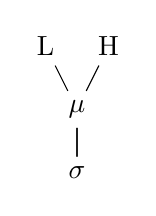
\begin{tikzpicture}[scale=0.8]
				\node (t1) at (1,1) {L};
				\node (t2) at (2,1) {H};
				\node (c2) at (1.5,0) {$\mu$};
				\node (s1) at (1.5,-1) {$\sigma$};
				\draw (t1) -- (c2) -- (s1);
				\draw (t2) -- (c2) -- (s1);
		\end{tikzpicture}} &
		
		\makecell[c]{\vspace{2pt}
			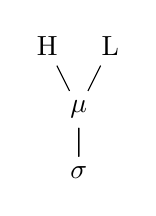
\begin{tikzpicture}[scale=0.8]
				\node (t1) at (1,1) {H};
				\node (t2) at (2,1) {L};
				\node (c2) at (1.5,0) {$\mu$};
				\node (s1) at (1.5,-1) {$\sigma$};
				\draw (t1) -- (c2) -- (s1);
				\draw (t2) -- (c2) -- (s1);
		\end{tikzpicture}} &
		
		\makecell[c]{\vspace{2pt}
			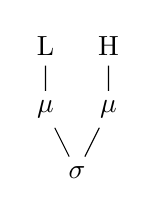
\begin{tikzpicture}[scale=0.8]
				\node (t1) at (1,1) {L};
				\node (t2) at (2,1) {H};
				\node (c1) at (1,0) {$\mu$};
				\node (c3) at (2,0) {$\mu$};
				\node (s1) at (1.5,-1) {$\sigma$};
				\draw (t1) -- (c1) -- (s1);
				\draw (t2) -- (c3) -- (s1);
		\end{tikzpicture}} &
		
		\makecell[c]{\vspace{2pt}
			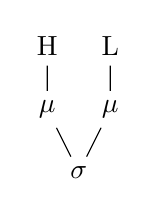
\begin{tikzpicture}[scale=0.8]
				\node (t1) at (1,1) {H};
				\node (t2) at (2,1) {L};
				\node (c1) at (1,0) {$\mu$};
				\node (c3) at (2,0) {$\mu$};
				\node (s1) at (1.5,-1) {$\sigma$};
				\draw (t1) -- (c1) -- (s1);
				\draw (t2) -- (c3) -- (s1);
		\end{tikzpicture}} \\
		\midrule
		Hausa & N & N & N & Y \\
		Mende & N & Y & Y & Y \\
		\bottomrule
	\end{tabular}
	\caption{Contour Inventory in Hausa and Mende}
	\label{tab.2typescontours}
\end{table}


There is more than one method to achieve this algorithmically.
We use a matrix-based containment checker to determine whether two 
ARs, even with the same tone sequence and the same number of syllable 
and mora, will have the same associations.

The matrix containment follows exactly parallel to the general notion
of any structural containment: matrix $A$ is \textit{contained} in
matrix $B$ if there exists a \textit{submatrix} of $B$, denoted $B'$,
that functions as a restriction discussed in Definition~\ref{def.res}, such that all
relations within $A$ are relatively preserved in correspondence with
those in $B'$, as in Definition~\ref{def.contain}.
The following two definitions (Definition~\ref{def.submatrix} and 
\ref{def.ar.matching}) specialize these concepts to the matrix 
representation of ARs.

\begin{definition}
	\label{def.submatrix}
	\textit{Let matrix $A$ be an $m \times n$ matrix.  Matrix $B$ is a
		\emph{submatrix}
		of $A$ by taking $k \ (1 \leq k \leq m)$ contiguous rows and $v \ (1 \leq v
		\leq n)$ contiguous columns from $A$.}\footnote{The term ``submatrix" is
		generally defined by deleting arbitrary rows and/or columns from the original
		matrix. However, in our case, we require a more restricted definition: the
		remaining rows and columns must be \textit{contiguous} in the original matrix,
		which reflects tonal locality.}
\end{definition}

\begin{definition}
	\label{def.ar.matching}
	\textit{
		An $m\times n$ matrix $A = [a_{ij}]$ is \emph{contained} in a matrix $B (A
		\sqsubseteq B)$, if there exists an $m\times n$ submatrix in B, denoted by $B' =
		[b'_{ij}]$ such that for all $i \in [0,m] ,j \in [0,n],\ b'_{ij}  \geq \ a_{ij}
		$.}
\end{definition}

Definition \ref{def.submatrix} defines what a submatrix is.  Definition
\ref{def.ar.matching}
states that a smaller matrix \( A = [a_{ij}] \) is contained in a larger matrix
\( B =
[b_{ij}] \) if we can find a submatrix \( B' \subseteq B \), with the same
dimensions as \( A \), such that the value of each entry in \( B' \) 
is at least as large as the corresponding entry in \( A \); that is, \(
b'_{ij} \geq a_{ij} \) for all \( i, j \). Since the entries of these matrices
are binary, this condition implies two cases:

\begin{enumerate}[label=(\alph*)]
	\item If \( a_{ij} = 1 \), meaning there is an association between node \(
	i \) and node \( j \) in the smaller matrix \( A \), then \( b'_{ij} \) must
	also be 1. This ensures an association found in \( A \) is preserved in \(B'\)
	at the same position;
	\item If \( a_{ij} = 0 \), meaning no association exists between node \( i \)
	and node \( j \) in the smaller matrix \( A \), then \( b'_{ij} \) may be
	either 0 or 1. In other words, \( B' \) may or may not have an
	association at the corresponding position. It is permitted to contain
	additional associations beyond those in \( A \), but it must not omit any that
	are present in \( A \).
\end{enumerate}

The comparison proceeds by first identifying whether the tonal string of one
structure is contained within another, and then verifying whether the
corresponding association matrices align. Even when a tonal substring match
is found, containment is established only if the associated tone--mora and
mora--syllable submatrices match within the aligned region. The full algorithm
is provided in the Supplementary Material, along with a detailed walk-through.
Figure~\ref{fig:matrixmatching} illustrates this procedure:
(\subref{fig:matrix-light}) is not contained in
(\subref{fig:matrix-heavy}) or (\subref{fig:matrix-super}),
whereas (\subref{fig:matrix-heavy}) is contained in
(\subref{fig:matrix-super}), since the submatrices in
(\subref{fig:matrix-super}) (the shaded cells) match the matrices of
(\subref{fig:matrix-heavy}) in terms of associations
as well as tonal strings, but do not match those of
(\subref{fig:matrix-light}).
\begin{figure}[ht]
\centering 
\setlength{\tabcolsep}{5pt}
% --- Block (a) ---
	\begin{subtable}[t]{0.25\textwidth}
		\centering
		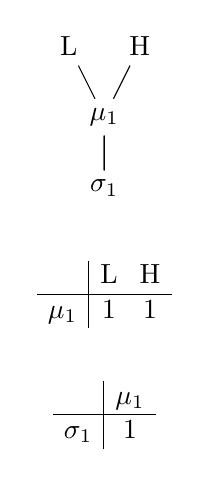
\begin{tikzpicture}[scale = 0.9]
			\node (bt1) at (1,1) {L};
			\node (bt2) at (2,1) {H};
			\node (bc1) at (1.5,0) {$\mu_1$};
			\node (bs1) at (1.5,-1) {$\sigma_1$};
			\draw (bt1) -- (bc1) -- (bs1);
			\draw (bt2) -- (bc1) -- (bs1);
			
			% Array 1 (b)
			\node (barray1) at (1.5,-2.5) {
			  \begin{tabular}{c|cc}
			    & L & H \\
			    \hline
			    $\mu_1$ & 1 & 1
			  \end{tabular}
			};
			
			% Array 2 (b)
			\node (barray2) at (1.5, -4.2) {
				\begin{tabular}{c|c}
					& $\mu_1$ \\
					\hline
					$\sigma_1$ & 1  
				\end{tabular}
				};
		\end{tikzpicture}
		\subcaption{}
		\label{fig:matrix-light}
	\end{subtable}
	\hfill
	% --- Block (B) ---
	\begin{subtable}[t]{0.25\textwidth}
		\centering
		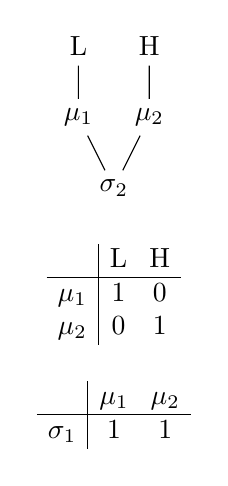
\begin{tikzpicture}[scale = 0.9]
			\node (ct1) at (1,1) {L};
			\node (ct2) at (2,1) {H};
			\node (cc1) at (1,0) {$\mu_1$};
			\node (cc2) at (2,0) {$\mu_2$};
			\node (cs1) at (1.5,-1) {$\sigma_2$};
			\draw (ct1) -- (cc1) -- (cs1);
			\draw (ct2) -- (cc2) -- (cs1);
			
			% Array 1
			\node (carray1) at (1.5, -2.5) {
				\begin{tabular}{c|cc}
					& L & H \\
					\hline
					$\mu_1$ & 1 & 0 \\
					$\mu_2$ & 0 & 1 
				\end{tabular}
				};
			
			% Array 2 
			\node (carray2) at (1.5, -4.2) {				
			\begin{tabular}{c|cc}
					& $\mu_1$ & $\mu_2$ \\
					\hline
					$\sigma_1$ & 1  & 1
				\end{tabular}};
		\end{tikzpicture}
		\subcaption{}
		\label{fig:matrix-heavy}
	\end{subtable}
	\hfill
	% --- Block (C) ---
	\begin{subtable}[t]{0.3\textwidth}
		\centering
		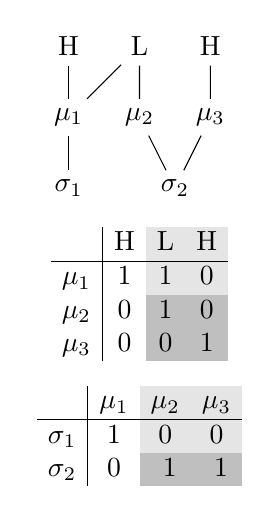
\begin{tikzpicture}[scale = 0.9]
			\node (dt0) at (0,1) {H};
			\node (dt1) at (1,1) {L};
			\node (dt2) at (2,1) {H};
			\node (dc0) at (0,0) {$\mu_1$};
			\node (dc1) at (1,0) {$\mu_2$};
			\node (dc2) at (2,0) {$\mu_3$};
			\node (ds0) at (0,-1) {$\sigma_1$};
			\node (ds1) at (1.5,-1) {$\sigma_2$};
			\draw (dt1) -- (dc1) -- (ds1);
			\draw (dt0) -- (dc0) -- (ds0);
			\draw (dt2) -- (dc2) -- (ds1);
			\draw (dt1) -- (dc0);
			
			% Array 1 (c)
			\node (darray1) at (1, -2.5) {
				\begin{tabular}{c|c>{\columncolor[gray]{0.9}}c>{\columncolor[gray]{0.9}}c}
					& H & L & H \\
					\hline
				$\mu_1$ & 1	&	1 & 0 \\
				$\mu_2$ & 0 & \cellcolor{gray!50}1 & \cellcolor{gray!50}0\\
				$\mu_3$ &0 &\cellcolor{gray!50}0&\cellcolor{gray!50}1\\
				\end{tabular}
				};
			
			% Array 2 (c)
			\node (darray2) at (1, -4.5) {
					\begin{tabular}
						{c|c>{\columncolor[gray]{0.9}}c>{\columncolor[gray]{0.9}}c}
					& $\mu_1$ & $\mu_2$ & $\mu_3$\\
					\hline
					$\sigma_1$ & 1 & 0 & 0\\
					$\sigma_2$ & 0 &  \cellcolor{gray!50} 1 & \cellcolor{gray!50} 1\\
				\end{tabular}
				};
		\end{tikzpicture}
		\subcaption{}
		\label{fig:matrix-super}
	\end{subtable}
	\hfill
	\caption{Light LH (11a), heavy LH (11b), 
	and a superfactor of heavy LH (11c)}
	\label{fig:matrixmatching}
\end{figure}


\subsection{Summary}
This section established BUFIA-AR, which and implementation 
of two functions that are core to the BUFIA-AR framework: 
\textsc{NextSupFact} and \textsc{Contain}, which are 
used in the case study described in the next section.


\section{Case Study: Hausa} \label{sec:hausa} is grounded in autosegmental 
theory. In particular, we explained the rationale

This section presents a case study applying BUFIA-AR to identify
tonotactic constraints over ARs in Hausa. We examine Hausa because
suitable data was available; we are unaware of a similar dataset for
Mende. The analysis focuses on non-derived native Hausa words,
examples of which are shown in Table~\ref{ex.hausa.words}. As mentioned
earlier, in Hausa monomoraic syllables can bear either H or L, but
cannot bear contours. A bimoraic syllable can take an HL contour (each
tone associates to one mora) but LH contours are not allowed. Lastly,
Hausa does not have superheavy syllables, therefore monosyllabic
three-tone contours are also not allowed.  


\begin{table}[h!]
	\centering
	\renewcommand{\arraystretch}{2}
	\begin{tabular}{lllll}
		\hline
		
		\textbf{Monosyllabic} 
		& \makecell{\textipa{\texthtd}áa \\ `son’} 
		& \makecell{mèe \\ `what’} 
		& \makecell{mâi \\ `oil’} 
		
		&  \\ \hline
		\textbf{Disyllabic} 
		& \makecell{\textipa{\texthtk}á.sáa \\ `land’} 
		& \makecell{mù.tûm \\ `person’} 
		& \makecell{tú.dùu \\ `hill’} 
		& \makecell{màa.gée \\ `cat’}  \\
		\hline
		
		\textbf{Trisyllabic} 
		& \makecell{í.nú.wàa \\ `shadow’} 
		& \makecell{\textipa{\texthtk}àn.\textipa{\texthtk}á.ráa \\ `ice/snow’} 
		& \makecell{múu.jì.yáa \\ `owl'} 
		& \makecell{fà.dá.màa\\ `swamp'} \\ \hline
	\end{tabular}
	\caption{Nonderived native Hausa words \citep{wold-4}}
	\label{ex.hausa.words}
\end{table}

\citet[p.606]{Newmanbook} notes
non-derived disyllabic words exhibit canonical normal tone
patterns: H.L, L.H, and H.H. For trisyllabic nouns, H.L.H,
H.H.L, L.H.L, and L.H.H are very common, but L.L.H is less
common with basic lexical items. Words ending in L.L, either 
disyllabic or polysyllabic words containing L.L, are relatively uncommon, 
especially when the second syllable bears a long vowel. 
When L.L forms do occur, they are typically restricted to 
ideophones or loanwords \citep[p.606]{Newmanbook}. 
\citet{zoll2003optimal} argues that the absence of H.L.L
and L.L.H is a result of the constraint \textsc{*Lapse} (which
forbids L from spreading across adjacent syllables) outranking
\textsc{*Clash} (which forbids H from spreading across two syllables).
In addition, for canonical, non-derived forms falling (F) tones 
typically fall on the last syllable \citep[p.606]{Newmanbook}.

Based on the above, the linguistically attested constraints in Hausa 
are summarised in Table~\ref{rules}, which are translated into 
AR constraints in Table~\ref{tab.rule.constraints}. In this 
study, we treat these constraints as the baseline grammar against which 
performance of BUFIA models is evaluated. Specifically, we investigate 
whether BUFIA-AR can accurately learn AR-based constraints, and 
if so, how the computationally attested constraints (henceforth, 
BUFIA constraints) correspond to previously identified linguistic 
ones (baseline constraints). We also include a BUFIA-string model 
as a comparison, which learns constraints over the same 
data using string representations.

\begin{table}
	\centering
	\begin{tabular}{ll}
		\toprule
		\textbf{Generalisations} & \textbf{Interpretation}                              \\
		\midrule
		\textbf{\textsc{*Rise$_\sigma$}}     & Syllables may not be associated with rising tones (LH) \\
		\textbf{\textsc{*Contour$_{\mu}$}}   & Moras may be associated with at most one tone.      \\
		\textbf{\textsc{*3t-Contour}}        & No trimoraic contour  \\
		\textbf{\textsc{*NonFinal-Fall}}     & No nonfinal HL contour for polysyllabic words         \\
		\textbf{\textsc{*Lapse}}             & No L spreading across syllables \\
		\bottomrule
	\end{tabular}
	\caption{Phonological Generalisations in Hausa}
	\label{rules}
\end{table}
\begin{table}
	\centering
	\begin{tabular}{ccccc}
		\toprule
		\textbf{\textsc{*Rise$_\sigma$}} &
		\textbf{\textsc{*Contour$_{\mu}$}} &
		\textbf{\textsc{*3t-Contour}} &  
		\textbf{\textsc{*NonFinal-Fall}} &
		\textbf{\textsc{*Lapse}} \\
		\midrule
		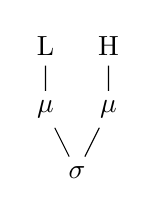
\begin{tikzpicture}
			\node (bt1) at (-.4,0.8) {L};
			\node (bt2) at (.4,0.8) {H};
			\node (bc1) at (-.4,0) {$\mu$};
			\node (bc2) at (0.4,0) {$\mu$};
			\node (bs1) at (0,-0.8) {$\sigma$};
			\draw (bt1) -- (bc1) -- (bs1);
			\draw (bt2) -- (bc2) -- (bs1);
		\end{tikzpicture} &
		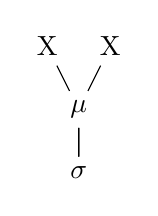
\begin{tikzpicture}
			\node (bt1) at (-.4,0.8) {X};
			\node (bt2) at (.4,0.8) {X};
			\node (bc1) at (0,0) {$\mu$};
			\node (bs1) at (0,-0.8) {$\sigma$};
			\draw (bt1) -- (bc1) -- (bs1);
			\draw (bt2) -- (bc1) -- (bs1);
		\end{tikzpicture} &
		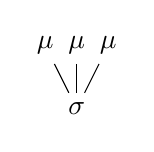
\begin{tikzpicture}
			\node (bt1) at (-.4,0.8) {$\mu$};
			\node (bt2) at (.0,0.8) {$\mu$};
			\node (bt3) at (.4,0.8) {$\mu$};
			\node (bs1) at (0,-0) {$\sigma$};
			\draw (bt1)  -- (bs1);
			\draw (bt2) -- (bs1);
			\draw (bt3) -- (bs1);
		\end{tikzpicture} &
		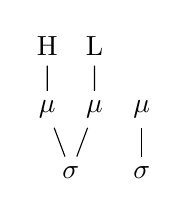
\begin{tikzpicture}
			\node (bt1) at (-.6,0.8) {H};
			\node (bt2) at (0,0.8) {L};
			\node (bc1) at (-.6,0) {$\mu$};
			\node (bc2) at (0,0) {$\mu$};
			\node (bs1) at (-.3,-0.8) {$\sigma$};
			\node (bc3) at (0.6,0) {$\mu$};
			\node (bs2) at (0.6,-0.8) {$\sigma$};
			\draw (bt1) -- (bc1) -- (bs1);
			\draw (bt2) -- (bc2) -- (bs1);
			\draw (bc3) -- (bs2);    
		\end{tikzpicture} &
		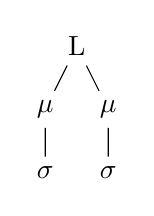
\begin{tikzpicture}
			\node (bt1) at (0,0.8) {L};
			\node (bc1) at (-.4,0) {$\mu$};
			\node (bc2) at (.4,0) {$\mu$};
			\node (bs1) at (-.4,-0.8) {$\sigma$};
			\node (bs2) at (.4,-0.8) {$\sigma$};
			\draw (bt1) -- (bc1) -- (bs1);
			\draw (bt1) -- (bc2) -- (bs2);
		\end{tikzpicture} \\
		\bottomrule
	\end{tabular}
	\caption{Phonological Generalisations Translated into forbidden ARs}
	\label{tab.rule.constraints}
\end{table}




\subsection{Experiment Setup}
The data used for the current experiment comes from the Hausa dataset
\citep{wold-4} in The World Loanword Database (WOLD) \citep{wold}. It
consists of around 1460 core words whose meanings are present in the
Loanword Typology meaning list. This list includes forms and concepts
that all languages have terms for. For the Hausa dataset, the
vocabulary contains 1668 core meaning-word pairs, along with other
information in fields titled Form, Meaning, Loanword Status, and
Analysability. To ensure consistency with previous generalisations, 
which are based on canonical, non-derived tonal patterns,
we restrict our dataset to monomorphemic words that are clearly 
non-borrowed, and all others were filtered out. In addition, forms 
containing glides (\textipa{\texthtk}w, \textipa{\texthtk}y, kw, ky, gw, gy) 
were excluded to avoid 
ambiguous syllabification and uncertain syllable weight.
As a result, a total of 621 words transcribed in orthography
remained and were stored in a .csv file.
All orthographic forms were first syllabified \citep{kodner2016} then
converted into its corresponding AR representation using the method
described in \citet{jardine2015concatenation}. 
Table~\ref{tab.conversion} shows how an orthographic form with
tonal markers is transformed into its corresponding matrix
representation. After conversion and removal of duplicate ARs, 64
distinct AR types were identified among the 621 words, which serve as
the positive dataset on which BUFIA-AR operates.
\begin{table}[ht]
	\centering
	\begin{tabular}{
			>{\centering\arraybackslash}m{1.2cm}|
			>{\centering\arraybackslash}m{1cm}|
			>{\centering\arraybackslash}m{3.2cm}|
			>{\centering\arraybackslash}m{8cm}
		}
		\toprule
		\textbf{Form} &
		\textbf{Tones} &
		\textbf{AR Diagram} &
		\textbf{Matrix-based Encodings} \\
		\midrule
		\makecell{\textit{k\`oo.g\'ii}\\`river'}
		&
		LH
		&
		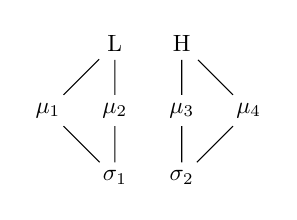
\begin{tikzpicture}[scale=.85,every node/.style={scale=.85}]
			\node (t1) at (2,1) {L};
			\node (t2) at (3,1) {H};
			
			\node (c1) at (1,0) {$\mu_1$};
			\node (c2) at (2,0) {$\mu_2$};
			\node (c3) at (3,0) {$\mu_3$};
			\node (c4) at (4,0) {$\mu_4$};
			
			\node (s1) at (2,-1) {$\sigma_1$};
			\node (s2) at (3,-1) {$\sigma_2$};
			
			\draw (t1)--(c1)--(s1);
			\draw (t1)--(c2)--(s1);
			\draw (t2)--(c3)--(s2);
			\draw (t2)--(c4)--(s2);
		\end{tikzpicture}
		&
		\[
		\begin{array}{c|cc}			
		& \text{ L } & \text{ H }\\
			\hline
			\mu_1 & 1 & 0\\
			\mu_2 & 1 & 0\\
			\mu_3 & 0 & 1\\
			\mu_4 & 0 & 1
		\end{array}
		\quad
		\begin{array}{c|cccc}
			& \,\mu_1\, &\,\mu_2 \,& \,\mu_3\, &\, \mu_4\,\\
			\hline
			\sigma_1 & 1 & 1 & 0 & 0\\
			\sigma_2 & 0 & 0 & 1 & 1
		\end{array}
		\]
		\\
		\midrule		
		\makecell{\textit{mù.tûm}\\`person'}
		&
		LF
		&
		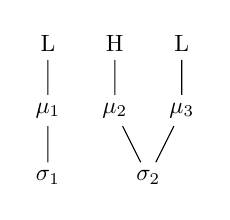
\begin{tikzpicture}[scale=.85,every node/.style={scale=.85}]
			\node (t0) at (1,1) {L};
			\node (t1) at (2,1) {H};
			\node (t2) at (3,1) {L};
			
			\node (c1) at (1,0) {$\mu_1$};
			\node (c2) at (2,0) {$\mu_2$};
			\node (c3) at (3,0) {$\mu_3$};
			
			\node (s1) at (1,-1) {$\sigma_1$};
			\node (s2) at (2.5,-1) {$\sigma_2$};
			
			\draw (t0)--(c1)--(s1);
			\draw (t1)--(c2)--(s2);
			\draw (t2)--(c3)--(s2);
		\end{tikzpicture}
		&
		\[
		\begin{array}{c|ccc}
			& \text{ L } & \text{ H } & \text{ L }\\
			\hline
			\mu_1 & 1 & 0 & 0\\
			\mu_2 & 0 & 1 & 0\\
			\mu_3 & 0 & 0 & 1
		\end{array}
		\quad
		\begin{array}{c|ccc}
			& \,\mu_1\, &\,\mu_2 \,& \,\mu_3\,\\
			\hline
			\sigma_1 & 1 & 0 & 0\\
			\sigma_2 & 0 & 1 & 1
		\end{array}
		\]
		\\		\bottomrule
	\end{tabular}
	
	\caption{Corresponding lexical forms, ARs, and their matrix-based encodings.}
	\label{tab.conversion}
\end{table}

We ran BUFIA-AR with the number of syllables,
moras, and tones limited to a maximum of three. 
The number three was chosen for two reasons. 
First, two of the baseline constraints in
Table~\ref{tab.rule.constraints} have three moras. 
If BUFIA-AR stopped searching for constraints before 
structures with three moras, it would not find those 
constraints. Second, we wanted to show that BUFIA-AR 
could return constraints with unassociated units, which 
is a unique aspect of ARs as compared to linear 
representations.

\subsection{Evaluation}
In this section, we provide two types of evaluation: qualitative and 
quantitative. The qualitative evaluation examines how the grammar learned 
by BUFIA-AR compares with the baseline grammar. The quantitative 
evaluation uses $k$-fold cross-validation,
a common method in machine learning for assessing 
how well a predictive model generalises to unseen data. 
\subsubsection{Qualitative Evaluation: Constraints Comparison}
BUFIA-AR found 11 constraints when the numbers of 
syllable, mora, and tone are limited to three. 
More generally, the output of BUFIA-AR for smaller 
values $s,\mu$ and the number of tones are subsets 
of the 11 constraints in Table~\ref{tab.results}. 
Cells with a dash indicate that no constraints were 
found with those $s$ and $\mu$ sizes.  

\begin{table}[hbt]
	\centering
	\begin{tabular}{c|c|c|c}
		\toprule
		& $\mu = 1$ & $\mu = 2$ & $\mu = 3$ \\
		\midrule
		$s = 1$ & 
		\begin{subtable}[t]{1.2cm}
			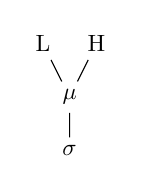
\begin{tikzpicture}[scale=.85,every node/.style={scale=.85}]
				\node (bt1) at (-.4,0.8) {L};
				\node (bt2) at (.4,0.8) {H};
				\node (bc1) at (0,0) {$\mu$};
				\node (bs1) at (0,-0.8) {$\sigma$};
				\draw (bt1) -- (bc1) -- (bs1);
				\draw (bt2) -- (bc1);
			\end{tikzpicture}
				\subcaption{}\label{cons.a}
			\end{subtable}
		\begin{subtable}[t]{1.2cm}
				\centering
			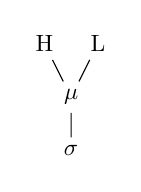
\begin{tikzpicture}[scale=.85,every node/.style={scale=.85}]
				\node (bt1) at (-.4,0.8) {H};
				\node (bt2) at (.4,0.8) {L};
				\node (bc1) at (0,0) {$\mu$};
				\node (bs1) at (0,-0.8) {$\sigma$};
				\draw (bt1) -- (bc1) -- (bs1);					
				\draw (bt2) -- (bc1);
			\end{tikzpicture}
				\subcaption{}
				\label{cons.b}
		\end{subtable}
			&
		\begin{subtable}[t]{1.2cm}
			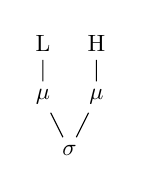
\begin{tikzpicture}[scale=.85,every node/.style={scale=.85}]
				\node (bt1) at (-.4,0.8) {L};
				\node (bt2) at (.4,0.8) {H};
				\node (bc1) at (-.4,0) {$\mu$};
				\node (bc2) at (.4,0) {$\mu$};
				\node (bs1) at (0,-0.8) {$\sigma$};
				\draw (bt1) -- (bc1) -- (bs1);
				\draw (bt2) -- (bc2) -- (bs1);
			\end{tikzpicture}
			\subcaption{}
			\label{cons.c}
		\end{subtable}
			&
		\begin{subtable}[t]{1.2cm}
		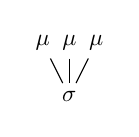
\begin{tikzpicture}[scale=.85,every node/.style={scale=.85}]
				\node (bc1) at (-.4,0) {$\mu$};
				\node (bc2) at (.4,0) {$\mu$};
				\node (bc3) at (0,0) {$\mu$};
				\node (bs1) at (0,-0.8) {$\sigma$};
				\draw (bc1) -- (bs1);
				\draw (bc2) -- (bs1);
				\draw (bc3) -- (bs1);
			\end{tikzpicture}
			\subcaption{}
			\label{cons.d} 
		\end{subtable}\\
		\midrule
		$s = 2$ & - & - &
		\begin{subtable}[t]{1.2cm}
			\begin{tikzpicture}[scale=.85,every node/.style={scale=.85}]
				\node (bt1) at (-.4,0.8) {H};
				\node (bt2) at (.4,0.8) {L};					
				\node (bc1) at (-.4,0) {$\mu$};
				\node (bc2) at (0,0) {$\mu$};
				\node (bc3) at (.4,0) {$\mu$};
				\node (bs1) at (-.4,-0.8) {$\sigma$};
				\node (bs2) at (.4,-0.8) {$\sigma$};
				\draw (bt1) -- (bc1) -- (bs1);
				\draw (bt2) -- (bc2) -- (bs1);
				\draw (bt2) -- (bc3) -- (bs2);
			\end{tikzpicture}\subcaption{}\label{cons.e}
		\end{subtable} \hfill
		\begin{subtable}[t]{1.2cm}
			\begin{tikzpicture}[scale=.85,every node/.style={scale=.85}]
					\node (bt1) at (-.4,0.8) {H};
					\node (bt2) at (.4,0.8) {L};
					\node (bc1) at (-.4,0) {$\mu$};
					\node (bc2) at (0,0) {$\mu$};
					\node (bc3) at (.4,0) {$\mu$};
					\node (bs1) at (-.4,-0.8) {$\sigma$};
					\node (bs2) at (.4,-0.8) {$\sigma$};
					\draw (bt1) -- (bc1) -- (bs1);
					\draw (bt1) -- (bc2) -- (bs2);
					\draw (bt2) -- (bc3) -- (bs2);
				\end{tikzpicture}
				\subcaption{}
				\label{cons.f}
		\end{subtable} \hfill
		\begin{subtable}[t]{1.2cm}
			\begin{tikzpicture}[scale=.85,every node/.style={scale=.85}]
					\node (bt1) at (0,0.8) {H};
					\node (bt2) at (.4,0.8) {L};
					\node (bt3) at (.8,0.8) {H};
					\node (bc1) at (-.4,0) {$\mu$};
					\node (bc2) at (0,0) {$\mu$};
					\node (bc3) at (.4,0) {$\mu$};
					\node (bs1) at (-.4,-0.8) {$\sigma$};
					\node (bs2) at (.4,-0.8) {$\sigma$};
					\draw (bt1) -- (bc1) -- (bs1);
					\draw (bt1) -- (bc2) -- (bs1);
					\draw (bt1) -- (bc3) -- (bs2);
			\end{tikzpicture}\subcaption{}\label{cons.g}
		\end{subtable}
		\\ \midrule
		$s = 3$ & - & - &
		\begin{subtable}[t]{1.2cm}
			\begin{tikzpicture}[scale=.85,every node/.style={scale=.85}]
				\node (bt1) at (-.4,0.8) {H};
				\node (bt2) at (.4,0.8) {L};
				\node (bc1) at (-.4,0) {$\mu$};
				\node (bc2) at (0,0) {$\mu$};
				\node (bc3) at (.4,0) {$\mu$};
				\node (bs1) at (-.4,-0.8) {$\sigma$};
				\node (bs2) at (0,-0.8) {$\sigma$};
				\node (bs3) at (.4,-0.8) {$\sigma$};
				\draw (bt1) -- (bc1) -- (bs1);
				\draw (bt2) -- (bc2) -- (bs2);					
				\draw (bt2) -- (bc3) -- (bs3);
			\end{tikzpicture}\subcaption{}\label{cons.h}
		\end{subtable}			\hfill
		\begin{subtable}[t]{1.2cm}
			\begin{tikzpicture}[scale=.85,every node/.style={scale=.85}]
				\node (bt1) at (-.4,0.8) {L};
				\node (bt2) at (0,0.8) {H};
				\node (bt3) at (.4,0.8) {L};
				\node (bc1) at (-.4,0) {$\mu$};
				\node (bc2) at (0,0) {$\mu$};					
				\node (bc3) at (.4,0) {$\mu$};
				\node (bs1) at (-.4,-0.8) {$\sigma$};
				\node (bs2) at (0,-0.8) {$\sigma$};
				\node (bs3) at (.4,-0.8) {$\sigma$};
				\draw (bt1) -- (bc1);
				\draw (bt1) -- (bc2);					
				\draw (bt1) -- (bc3);
				\draw (bc1) -- (bs1);
				\draw (bc2) -- (bs2);
				\draw (bc3) -- (bs3);
			\end{tikzpicture}\subcaption{}\label{cons.i}
		\end{subtable}  \hfill
		\begin{subtable}[t]{1.2cm}
			\begin{tikzpicture}[scale=.85,every node/.style={scale=.85}]
				\node (bt1) at (-.4,0.8) {H};
				\node (bt2) at (0,0.8) {L};
				\node (bt3) at (.4,0.8) {H};					
				\node (bc1) at (-.4,0) {$\mu$};
				\node (bc2) at (0,0) {$\mu$};
				\node (bc3) at (.4,0) {$\mu$};
				\node (bs1) at (-.4,-0.8) {$\sigma$};
				\node (bs2) at (0,-0.8) {$\sigma$};					
				\node (bs3) at (.4,-0.8) {$\sigma$};
				\draw (bt1) -- (bc1);
					\draw (bt1) -- (bc2);
				\draw (bc1) -- (bs1);
				\draw (bc2) -- (bs2);
				\draw (bc3) -- (bs3);
			\end{tikzpicture}\subcaption{}\label{cons.j}
		\end{subtable}  \hfill
		\begin{subtable}[t]{1.2cm}
			\begin{tikzpicture}[scale=.85,every node/.style={scale=.85}]
					\node (bt1) at (-.4,0.8) {L};
					\node (bt2) at (0,0.8) {H};
					\node (bt3) at (.4,0.8) {L};
					\node (bc1) at (-.4,0) {$\mu$};
					\node (bc2) at (0,0) {$\mu$};
					\node (bc3) at (.4,0) {$\mu$};
					\node (bs1) at (-.4,-0.8) {$\sigma$};
					\node (bs2) at (0,-0.8) {$\sigma$};
					\node (bs3) at (.4,-0.8) {$\sigma$};
					\draw (bt1) -- (bc1);
					\draw (bt2) -- (bc2);
					\draw (bt2) -- (bc3);
					\draw (bc1) -- (bs1);
					\draw (bc2) -- (bs2);
					\draw (bc3) -- (bs3);
				\end{tikzpicture}
				\subcaption{}
				\label{cons.k}
			\end{subtable}\\
	\bottomrule
	\end{tabular}
	\caption{Hausa constraints returned by BUFIA-AR  when $s \leq 3, \   t \leq 3, \ \mu \leq 3$}
	\label{tab.results}
\end{table}



As shown in Table~\ref{sec5.tab.compare}, all of these
constraints together constitute three categories: one where the
baseline constraints have matching BUFIA constraints, one where the
baseline constraints do not have corresponding BUFIA constraints, and
one where BUFIA constraints do not have corresponding baseline
constraints. In Table~\ref{sec5.tab.compare}, this third category of
constraints also provides names for the BUFIA constraints
(\ref{cons.e}-\ref{cons.h}) in terms of the melody and syllabification
implicated by the structures in Figure~\ref{tab.results}. Boldface 
indicates the tone on heavy syllables. These labels serve only 
as shorthand for the ARs shown in Table~\ref{sec5.tab.compare} and 
may be ambiguous, as they do not fully capture the structures. 

\begin{table}[h!]
	\centering
	\begin{tabular}{p{4cm}p{3.5cm}p{3.5cm}}
		\toprule
		\textbf{Present in both \newline BUFIA and Baseline} 
		& \textbf{Baseline Constraints \newline Absent from BUFIA} 
		& \textbf{BUFIA Constraints \newline Absent from Baseline} \\
		\midrule
		\textsc{*Rise}$_\sigma$~(\ref{cons.c})\newline
		\textsc{*Contour}$_\mu$~(\ref{cons.a}--\ref{cons.b})\newline
		\textsc{*3T-Contour}~(\ref{cons.d})\newline
		& \textsc{*NonFinal-Fall}\newline
		\textsc{*Lapse}
		& \textsc{*F.L}~(\ref{cons.e})\newline
		\textsc{*H.F}~(\ref{cons.f})\newline
		\textsc{*\textbf{H}.H-LH}~(\ref{cons.g})\newline
		\textsc{*H.L.L}~(\ref{cons.h})\newline
		\textsc{*L.L.L-HL}~(\ref{cons.i})\newline
		\textsc{*H.H-LH}~(\ref{cons.j})\newline
		\textsc{*L.H.H-L}~(\ref{cons.k})\\
		\bottomrule
	\end{tabular}
	\caption{Comparing baseline constraints with BUFIA constraints}
	\label{sec5.tab.compare}
\end{table}

The first category is when the BUFIA-AR attested constraints align
with the linguistic generalisations previously argued for in the
literature. For monosyllabic forms (when \(s=1\)), BUFIA-AR returned
four constraints: a monomoraic LH (\ref{cons.a}), a monomoraic HL
(\ref{cons.b}), a bimoraic LH (\ref{cons.c}), and a trimoraic
structure (\ref{cons.d}).  Each of these matches a baseline
constraint.  In particular, (\ref{cons.a}) and (\ref{cons.b}) together
account for the absence of monomoraic contour tones, or the constraint
\textsc{*Contour}$_\mu$. The two constraints further rule out any
structures in which a single mora associates with more than two
tones. Secondly, the BUFIA-constraint (\ref{cons.c}) precisely forbids 
a heavy LH contour, which is identical to \textsc{*Rise} constraint in
Table~\ref{tab.rule.constraints}. Its counterpart, a heavy HL
syllable, is not returned, which appropriately addresses the contour
asymmetry problem discussed earlier. Finally, (\ref{cons.d}) correctly
disallows trimoraic syllables as expressed by the constraint
\textsc{*3T-Contour}. BUFIA-AR does not return any specific tonal
forms for this structure, since any tonal sequence it carries will
ultimately violate the forbidden structure.
One thing to note here is that both \textsc{Contour}{$_\mu$} and
\textsc{3T-Contour} describe structural information:
\textsc{Contour}{$_\mu$} prohibits binary branching on a mora node,
while \textsc{3T-Contour} prohibits ternary branching on a syllable
node. The reason that \textsc{3T-Contour} can be ruled out by a single
constraint \ref{cons.d}, whereas two constraints, \ref{cons.a} and
\ref{cons.b}, are needed to account for \textsc{Contour}{$_\mu$} is
that in the current implementation, tonal specifications must be fully
specified, and we did not include an umbrella feature, or permit
under-specified tonal nodes, that would match both H and L.
Overall, BUFIA constraints (\ref{cons.a}-\ref{cons.d}) correctly
reflect frequently reported patterns regarding the tonal inventory,
TBU, and syllable weight, and arguably cover some of the most
fundamental aspects of Hausa tonology. This demonstrates that BUFIA-AR
is not only capable of learning these tonotactic patterns but also
expressing them in terms of ARs.
The second category regards baseline constraints without matching
BUFIA constraints. There are two of these constraints,
\textsc{*NonFinal-Fall} and \textsc{*Lapse}. Each of these appear to
be partially, not totally, accounted for by some of the BUFIA
constraints. For example, constraint~(\ref{cons.e}) partially captures
the generalisation \textsc{*NonFinal-Fall}, which requires that HL
contours do not occur in non-final position, and in particular, when
the following syllable bears a L tone. This is a clue that the BUFIA
constraints appear to allow for the possibility of an HL contour
followed by a H syllable because no constraint banning such a
configuration was returned. Indeed, a reverse search revealed six
words that exhibit these structures, as shown in Example 
(\ref{hlhwords}).\footnote{\citet[p.~607]{Newmanbook} lists eight
	non-derived words with an initial HL tone, possibly reflecting the
	historical loss of a low-tone vowel. The word \textit{kûn.née} `the ear'
	is one of
	these; the others did not appear in Newman’s records.} These
data points indicate that the constraint \textsc{*NonFinal-Fall} is
too strong and it must be further refined if it is to account for the
full range of observed data.
\ex Hausa words exhibiting HL.H pattern (\textsc{*NonFinal-Fall})

\label{hlhwords}
\setlength{\tabcolsep}{0pt} % reduce horizontal padding
\renewcommand{\arraystretch}{1} % single spacing
\begin{tabular}{@{}l@{\hspace{0.8em}}l@{\hspace{1em}}l@{}}
	a. & jîn.\textipa{\texthtk}ái        & ``the pity’’ \\
	b. & kûn.née        & ``the ear’’ \\
	c. & tsûm.máa       & ``the handkerchief or rag’’ \\
	d. & sâi.wáa        & ``the root’’ \\
	e. & bâu.táa        & ``worship’’ \\
	f. & yân.yáa.wàa    & ``the fox (fennec of Sahara)’’ \\
\end{tabular}
\xe


Consider the next baseline constraint \textsc{*Lapse}, which disfavours
the L-tone spreading, therefore predicts the absence of H.L.L and L.L.H 
\citep{zoll2003optimal}. The BUFIA constraint
(\ref{cons.h}) *H.L.L bans one form of H.L.L when all three syllables
are monomoraic, but does not entail banning other H.L.L structures, 
such as ones that contain a heavy syllable. An
example in the data is the word \textit{sá.bòo.dà} `because.' Even
though this word expresses the H.L.L pattern, it does not contain the
structure shown in (\ref{cons.h}) and therefore it satisfies BUFIA
constraint (\ref{cons.h}) *H.L.L.\footnote{Visually, \raisebox{-.4em}{
		\begin{tikzpicture}[scale=1,baseline=(current bounding box.center)]
			\node (bt1) at (-0.4,0.8) {\scriptsize H};
			\node (bt2) at (0.4,0.8) {\scriptsize L};
			\node (bc1) at (-0.4,0) {\scriptsize $\mu_1$};
			\node (bc2) at (0,0) {\scriptsize $\mu_2$};
			\node (bc3) at (0.4,0) {\scriptsize $\mu_3$};
			\node (bs1) at (-0.4,-0.8) {\scriptsize $\sigma_1$};
			\node (bs2) at (0,-0.8) {\scriptsize $\sigma_2$};
			\node (bs3) at (0.4,-0.8) {\scriptsize $\sigma_3$};
			\draw (bt1) -- (bc1) -- (bs1);
			\draw (bt2) -- (bc2) -- (bs2);
			\draw (bt2) -- (bc3) -- (bs3);
		\end{tikzpicture}
	}
	might appear to be contained in
	\raisebox{-.4em}{
		\begin{tikzpicture}[scale=1,baseline=(current bounding box.center)]
			\node (bt1) at (-0.4,0.8) {\scriptsize H};
			\node (bt2) at (0.4,0.8) {\scriptsize L};
			\node (bc1) at (-0.4,0) {\scriptsize $\mu_1$};
			\node (bc2) at (0,0) {\scriptsize $\mu_2$};
			\node (bc3) at (0.4,0) {\scriptsize $\mu_3$};
			\node (bc4) at (0.8,0) {\scriptsize $\mu_4$};
			\node (bs1) at (-0.4,-0.8) {\scriptsize $\sigma_1$};
			\node (bs2) at (0,-0.8) {\scriptsize $\sigma_2$};
			\node (bs3) at (0.8,-0.8) {\scriptsize $\sigma_3$};
			\draw (bt1) -- (bc1) -- (bs1);
			\draw (bt2) -- (bc2) -- (bs2);
			\draw (bt2) -- (bc3) -- (bs2);
			\draw (bt2) -- (bc4) -- (bs3);
		\end{tikzpicture}
	}
	but in fact the two structures are incomparable in the partially-ordered
	space because \(\mu_3\) is associated to \(\sigma_3\) in the former
	but not in the latter.}

Furthermore, BUFIA-AR did not return a constraint prohibiting the
factor L.L.H. In fact, there are also instances of this pattern as
shown in Example~(\ref{llhwords}). 

\ex Hausa words exhibiting the L.L.H pattern
\label{llhwords}

\begin{tabular}{@{}l@{\hspace{0.8em}}l@{\hspace{1em}}l@{}}
	a.  & mà.là.fáa      & ``the hat or cap’’ \\
	b.  & tùn.kù.yáu     & ``the flea’’ \\
	c.  & gì.zàa.góo     & ``the adze’’ \\
	d.  & tàu.ràa.róo    & ``the star’’ \\
	e.  & gàa.jì.màa.rée & ``the cloud’’ \\
\end{tabular}
\xe

To summarise, the reason BUFIA did not find the baseline constraints
\textsc{*NonFinal-Fall} and \textsc{*Lapse} is simply because they are
not true of the data, which has multiple forms violating those
constraints.

This brings us to the third category, which includes BUFIA constraints
without matching baseline constraints. Generally, these constraints
partially match \textsc{*NonFinal-Fall} and \textsc{*Lapse}. However,
since both baseline constraints are not generally true of the data,
the BUFIA constraints are typically more specific refinements of them,
forbidding narrower classes of forms. We can classify these constraints
to two types: constraints concerning contour (\ref{cons.e}, \ref{cons.f})
and constraints concerning spreading (\ref{cons.g}, \ref{cons.i},
\ref{cons.j}, \ref{cons.k}).

Constraint (\ref{cons.e}) and (\ref{cons.f}) specify two environments that forbid 
a HL contour: when a HL syllable is followed by a light L-toned syllable 
(\ref{cons.e}, *F.L), or when it is preceded by a light H-toned syllable 
(\ref{cons.f}, *H.F). The forms of F.L and H.F, termed as ``non-contrasting'' 
tone by \citet{zoll2003optimal}, have been reported in other languages. 
For instance, in Mende, disyllabic R.H undergoes tone absorption and
simplifies to L.H, and F.L simplifies into H.L \citep{leben2017tone}. 
In Hausa, since the light syllables with rising tones are banned, BUFIA-AR 
only returns *F.L and *H.F constraints. \citet[p.598]{Newmanbook} 
points out that F.L optionally changes to H.L in complex relative pronouns 
and adverbs; however, such simplification does not apply to our dataset, 
with which BUFIA-AR remains consistent.

In terms of the constraints concerning spreading, traditional OT includes 
\textsc{*Clash} and \textsc{*Lapse}, which ban adjacent syllables linked 
to either H or L. Among BUFIA constraints, \textsc{*Clash } and \textsc{*Lapse} 
are reflected in more specific forms as in constraint (\ref{cons.g}-\ref{cons.k}).

Constraints (\ref{cons.e}, *F.L), (\ref{cons.h}, *H.L.L), and (\ref{cons.i}, 
*L.L.L-HL) address the cases which forbid L spreading in particular 
circumstances. Constraint \kuo{cons.e} and \kuo{cons.h} prevent it after H 
tones, and \kuo{cons.i} prevents a trisyllabic L span before a HL melody.

Similarly, the constraint (\ref{cons.f}, *H.F), (\ref {cons.g}, *\textbf{H}.H-LH), 
(\ref{cons.j}, *H.H-LH), and (\ref{cons.k}, *L.H.H-L) restrict H-spreading 
in different environments. For example, \kuo{cons.g} and \kuo{cons.j} prohibit 
an H tone (preceding an LH) from spreading across two syllables, while 
\kuo{cons.k} forbids an H tone from spreading to two syllables when it is 
wedged between two L-toned syllables.

Finally, four BUFIA constraints (\ref{cons.g},*\textbf{H}.H-LH), 
(\ref{cons.i},*L.L.L-HL), (\ref{cons.j},*H.H-LH), and (\ref{cons.k},*L.H.H-L)
potentially demonstrate the expressive advantage of ARs over string
representations. These constraints involve unassociated units, either
unassociated tones or syllables. For example, Constraint
\kuo{cons.g} describes the following condition: when a H spreads over a heavy
syllable to another syllable, the tonal tier can only be extended by
adding one more tone. The association of the unassociated tones does not
have to be specified. A similar pattern is seen in \kuo{cons.i} where
if L tone spreads over three light syllables, the tonal tier will only
accommodate one more tone. These patterns reflect a central fact
regarding autosegmental phonology: units from different tiers do not
need to be synchronised. This idea is more difficult to express with
purely linear string representations.

In summary, this subsection reports the qualitative evaluation of 
BUFIA-AR by comparing BUFIA constraints with the constraints reported
by linguists. It was found that BUFIA-AR is able to learn tonotactic
patterns over AR, and that there are interesting differences between
the constraints produced by BUFIA-AR and those posited by earlier
researchers.


\subsubsection{Quantitative Evaluation: Cross-validation}

The $k$-fold cross-validation procedure partitions the dataset into 
$k$ folds. In each iteration, BUFIA-AR is trained on $k-1$ folds 
and evaluated on the remaining held-out fold. This process is 
repeated $k$ times so that each fold serves as the evaluation 
set exactly once.

Since BUFIA is a deterministic categorical learner, the distinction 
between token- and type-based datasets does not ultimately affect the 
learned grammar. However, we report both settings for completeness. 
In the type-based setting, the dataset consists of 
64 distinct Hausa AR types, randomly divided into four folds (16 types
per fold), with 48 used for training and 16 for testing. In the token-based setting, the full dataset of 621 
tokens is also randomly divided into four folds (155/156 per fold). Within 
the train set (465/466 in total), there were 55–62 unique types.

In each round, BUFIA-AR is trained on three folds and evaluated on the 
remaining fold. The baseline grammar is evaluated on the same held-out 
fold. Accuracy is defined as the proportion of correctly accepted forms in the held-out set (also known as \textit{recall}).

In addition, we apply the same procedure using a string-based 
version of BUFIA (BUFIA-Str). Both BUFIA-AR and BUFIA-Str require a user-defined complexity 
bound, which determines the maximum size of constraints considered 
by the algorithm. However, this notion of complexity is not directly 
comparable across representations. For BUFIA-AR, it is controlled 
by multiple parameters ($t, m, s$) that limit different tiers; 
we set these to $t = m = s = 3$ to match the constraints found in 
\ref{tab.results}. BUFIA-Str uses a single complexity 
parameter $k$. Since the maximum constraint length in 
Table~\ref{sec5.tab.compare} is $7$ (i.e. \ref{cons.j}), we set $k = 7$
to match this bound. This setting allows us to assess whether 
constraints identified over AR can also be recovered using a 
string-based representation under a comparable complexity limit.

\begin{table}
	\centering
	\setlength{\tabcolsep}{4pt}
	\begin{tabular}{ccccccccccc}
		\toprule
		& \multicolumn{4}{c}{\textbf{Type-Based}} & \multicolumn{4}{c}{\textbf{Token-Based}} \\
		\cmidrule(lr){2-5} \cmidrule(lr){6-9}
		\textbf{Fold} 
		& \textbf{Train/Test}
		& \textbf{AR} & \textbf{Str} & \textbf{Baseline}
		& \textbf{Train/Test}
		& \textbf{AR} & \textbf{Str} & \textbf{Baseline} \\
		\midrule
		
		1 & 48/16 
		& 0.938 & 0.500 & 0.812
		& 465/156 
		& 0.987 & 0.949 & 0.936 \\
		
		2 & 48/16 
		& 0.875 & 0.500 & 0.812
		& 466/155
		& 0.994 & 0.974 & 0.942 \\
		
		3 & 48/16 
		& 0.875 & 0.812 & 0.938
		& 466/155
		& 1.000 & 1.000 & 0.955 \\
		
		4 & 48/16 
		& 0.938 & 0.812 & 0.688
		& 466/155
		& 0.994 & 0.942 & 0.974 \\
		
		\midrule
		\textbf{Avg} 
		& 
		& \textbf{0.907} & \textbf{0.656} & \textbf{0.812}
		& 
		& \textbf{0.994} & \textbf{0.966} & \textbf{0.952} \\
		
		\bottomrule
	\end{tabular}
	\caption{Four-fold cross-validation in both type- and token-based settings. In the token setting, the number of distinct types in Train are indicated in parentheses.}
	\label{sec4.tab.crosvalid}
\end{table}


As shown in Table~\ref{sec4.tab.crosvalid}, BUFIA-AR outperforms
BUFIA-Str and the baseline grammar, and reaches an average accuracy of 0.907 
in the type-based setting and 0.994 in the token-based setting. 
The overall performance increase in the token-based setting is expected because of the uneven distribution of tokens over types: most types are rare \citep{Yang2013}. Consequently, frequently attested structures are likely to be attested in training and form a larger proportion of the testing data.

BUFIA-Str performs below the baseline in the type-based 
setting (0.656 < 0.812), but outperforms in the token-based setting 
(0.966 > 0.952). The lower performance in the 
type-based setting is likely due to the relatively high complexity 
threshold ($k=7$), which leads to overfitting in the type-based setting.
In the token-based setting, this effect is compensated.
These results suggest that the BUFIA-AR supports 
stronger generalisation over distinct types, including rare ones,
even without frequency information.

In addition, across all four folds, BUFIA-AR consistently 
returns the constraints (\ref{cons.a}–\ref{cons.f}) and (\ref{cons.h}), 
while the remaining constraints vary slightly across folds.
Altogether, this indicates that BUFIA-AR not only captures the core
generalisations of Hausa tonotactics but also extends to rarer and
more exceptional patterns that the baseline fails to account
for. Overall, the quantitative evaluation demonstrates that BUFIA-AR
generalises robustly to unseen data and empirically outperforms
a similar algorithm using string representations
and a theoretically motivated baseline grammar.


\section{Discussion}
\label{sec:discussion}

\subsection{Optimisation versus Satisfaction}
\label{sec:discussion.ot}
The grammars output by BUFIA-AR compute the well-formedness of a word
by checking whether its structure \textit{contains} any forbidden
structures (the negative literals), or equivalently, whether it
\textit{satisfies} all of the constraints. This is in contrast to
globally \textit{optimising} over \textit{violable} constraints.  The
pattern obtained by satisfying the 11 BUFIA constraints captures the
asymmetric distribution of spreading and contour formation while
accommodating the rarer data points. On the other hand, In
\citet{zoll2003optimal}’s Optimal Tone Mapping program, tonal mapping
arises from the optimisation over morphological directionality
constraints (\textsc{Align-R} and \textsc{Align-L}) and
quality-sensitive markedness constraints (\textsc{*Clash} and
\textsc{*Lapse}).

What are we to make of these differences? Consider how each approach explains the
common absence of non-contrasting forms such as
\textsc{*F.L} and \textsc{*H.F}.   Optimal Tone Mapping utilises
\textsc{*Clash} and \textsc{*Lapse} to help explain the absence of these unattested 
forms. Zoll observes this is an improvement over the traditional mapping approach, 
which explained their absence by the lack of a motivation for spreading. 
\citet{zoll2003optimal} writes, ``with one-to-one linking built into the Association 
Convention, nothing automatically forces one tone to
spread onto a syllable that already bears tone.''
On the other hand, BUFIA-AR returns no \textsc{*Lapse} or \textsc{*Clash} 
constraints, but instead returns more specific versions of them. 
There appears to be a trade-off between optimisation-based grammars using simpler 
constraints and satisfaction-based grammars using more complex constraints. 
One may then prefer optimisation-based grammars over satisfaction-based ones on the 
grounds that its constraints are simpler.

However, we argue that such a conclusion is premature. First, from a computational 
perspective, this trade-off may not be as significant as it appears because the 
phonological patterns being described are ultimately finite-state 
\citep{karttunen1998proper} or subregular \citep{Heinz-2011-CPF, Heinz-2011-CPGLF}. 
There are many ways to decompose a phonological pattern into parts, and it has been 
argued that understanding each of these ways is valuable \citep{Lambert-2025}.

Second, it is also the case that the dataset obtained from
\citet{wold-4} shows that Zoll's (2003) proposal, as it is presented,
cannot adequately capture the exceptional data points in the dataset
because *\textsc{Lapse} is undominated. Zoll acknowledges in footnote
18 that exceptions to the general pattern in Hausa could be
accommodated by a prespecificational account
\citep{inkelas1993inalterability}. However, another alternative that
Zoll does not consider would be to add to the grammar refined versions
of *\textsc{Lapse} like the ones that BUFIA-AR found.  In other words,
even optimisation-based grammars would benefit from more complex
constraints of the variety found by BUFIA-AR.

One objection to this latter approach is that it stands in opposition
to a core idea behind Optimality Theory, which is that CON is a
universal set of simple constraints and all language-specific
variation is a product of the interaction of these constraints via
ranking. Under this perspective the only learning that needs to take
place regards the ranking of the constraints
\citep{TesarSmolensky1998, TesarSmolensky2000}. This argument is fine
as far as it goes, but we are aware of no theory of CON which provides
a simplicity criterion its constraints must satisfy.

It is also the case that more recent research has shown how
constraints themselves can be learned from examples
\citep{hayes2008maximum, Heinz2009, Heinz2010, Lambert+2021-TESRL}.
This line of work coheres with the idea that not all constraints in
all languages are universal, and that some are in fact
learned. Provided a theory of generative grammar admits the learning
of some language-specific constraints, it is not clear to us why it
would be a problem for language-specific constraints that are a little
more complex than the ones attributed to CON to be included in a
grammar.

In this regard, it is important to point out that BUFIA-AR
does not return arbitrarily complex constraints. 
The collection of constraints output by BUFIA-AR forms a grammar which
corresponds to a particularly weak form of logic (the conjunction of
negative literals), and the structures themselves (ARs) are representations well-motivated by linguistic theory.

In sum, the debate between optimisation-based and satisfaction-based
approaches is one with a long history (see for example
\citet{Simon1956}), and will not likely be settled soon. Nonetheless,
the fact remains that BUFIA-AR returns a set of inviolable constraints
consistent with the data comparable to the ones utilised in earlier
analyses.

\subsection{Gradience versus Categoricity in Grammars}
\label{sec:discussion.grammar}

Another ongoing debate in phonotactic learning concerns whether the
grammar should be categorical or gradient. Learning models like
BUFIA(-AR) make clear distinctions between what is well-formed and
what is not since constraints are inviolable. By contrast, gradient
learning models, such as MaxEnt \citep{hayes2008maximum, GouskovaGallagher2020} discussed in Section~\ref{sec:learning.models},
treat constraints as \textit{weighted}. In these models,
Constraints extracted from a lexicon are assigned with probabilistic weights that correspond to well-formedness judgements
from native speakers, with lower probabilities representing lower degrees
of acceptability. In this line of research, gradience is inherent to
the grammar, and probabilistic induction is seen as inevitable for
phonotactic learning \citep{hayes2008maximum, wilson2018accidental}.

We argue that the absence of probabilistic induction in BUFIA-AR
should not be regarded as a deficiency for two main reasons.  First,
whether weights are \textit{necessary} in learning or in the grammar
remains a matter of debate. Second, although the presented
implementation of BUFIA-AR is categorical, it can be augmented with
probabilistic values if a gradient model is desired in certain
learning scenarios.

Regarding the first point, several lines of argument have challenged
the view that phonotactic grammars are gradient. Directly equating
probability with well-formedness, as \citet{hayes2008maximum} do, has
been argued to be mistaken because unlikely outcomes can still be
well-formed and likelihood ultimately decreases as size increases, but
well-formedness does not \citep{heinz2017computational}. Others have
argued that gradience in acceptability judgements may stem from
performance-related factors, such as misperception
\citep{kahng2023can} or psycholinguistic processing
\citep{Gorman2013}. Additionally, there is some evidence that
categorical models can perform just as well as, and sometimes even
better than, gradient models \citep{Gorman2013, Durvasula2020,
	KostyszynHeinz2021, Dai2025, Swanson+2025,durvasula2025closer}. For
example, \citet{Swanson+2025} conducted a comparative study between
BUFIA and MaxEnt on Quechua \citep{wilson2018accidental} and obtained
comparable results. \citet{durvasula2025closer} demonstrates that when
MaxEnt weights are either equalised or entirely removed, the model can
actually yield stronger predictions. Other recent studies further
highlight the versatility of categorical learners:
\citet{payne2024generalized} shows how BUFIA can be modified to learn
positive grammars, while \citet{Dai2025} proposes a categorical
learning model capable of filtering out exceptions.

Another point of view that has been expressed is that the
gradient/categorical distinction is not intrinsic to phonotactic
learning or the phonotactic grammar itself, but only differs in how
grammars assign values to constraints. In other words, the categorical
and gradient approaches can be analysed the same way; only the values
that a learner or grammar associates with constraint evaluation
changes \citep{goodman1999semiring, chandlee2017computational,
	mayerReconciling2025}. We are sympathetic to this view because this
reconciliation foregrounds grammatical structure and backgrounds the
particularities of the values. The values (whether binary, scalar, or
real) are details, but the grammatical structure itself is
paramount. This is precisely what theoretical computational studies
strive to elucidate \citep{heinzComputationalNaturePhonological2018}.

This is why it is worth noting that the current categorical learning
model of BUFIA-AR can be flexibly extended into a gradient learning
model. Doing so only requires that a different value-assigning
function be applied to the constraints. Accordingly, the current
BUFIA-AR model can be adapted into a gradient version in multiple
ways. Weights could be assigned to constraints obtained by BUFIA-AR on
the basis of any number of calculations including frequency of the
factors, their expected frequency, or based on a regression fit to
these or related numbers. Another approach would be to make the ARs
themselves gradient. In the current implementation, the binary values
(0/1) in the matrices simply represent the presence or absence of
association lines, which treats all types of associations in one of
these two ways. These binary values can be replaced with probabilistic
values of specific associations, so as to get a gradient grammar
\citep{SmolenskyGoldrick2013, Mayer2021}.

Finally, we emphasise that, despite the long-standing
shift in tonal phonology from segment/feature-based representations to
non-linear representations, existing gradient learning models do not,
as far as we are aware, operate directly over non-linear
representations such as ARs. We believe that it will be easier to
obtain a gradient tonotactic learning algorithm over ARs by modifying
BUFIA-AR as opposed to adapting existing string-based gradient
learning models to ARs.

In sum, the categorical nature of BUFIA-AR does not prohibit it from
being an important contribution to our understanding of how tonotactic
patterns can be learned.

\section{Conclusion}
\label{sec:conclusion}
This paper presents the first tonotactic learning algorithm over
autosegmental representations to our knowledge. Through a case study
of Hausa, we constructed a database containing 64 distinct ARs from
621 surface-true Hausa words and discovered, using BUFIA-AR, a
tonotactic constraint grammar consisting of 11 constraints (limited to
three syllables, three tones, and three moras). Furthermore, by
comparing BUFIA constraints with the baseline constraints, we found
partial overlaps: in some cases, the two matched, but more often the
BUFIA constraints were more specific. We also found data points in
conflict with previous analyses, and identified novel patterns not
previously reported in the linguistic literature, such as certain
constraints prohibiting tone spreading and contour formation in
particular environments. These findings demonstrate both the
feasibility of tonotactic grammar inference over ARs and the
advantages of using algorithmic approaches to refine and extend
earlier generalisations.

Another contribution of this paper is the modelling of ARs, including
their expansion and containment checking, in a manner that is both
computationally efficient and linguistically faithful. The pipeline 
employed in this study, from data preparation and orthography-to-AR 
conversion to the implementation of BUFIA-AR, can serve as a general 
tool for exploring tonotactic constraints in other languages, and as 
a foundation for future work on more complex tonal process learning.

There are several directions for future research. It would be valuable
to investigate the psychological reality of the constraints inferred
by BUFIA-AR, seeking external evidence from cognition and perception
studies. Such evidence could bear on the stopping criteria for
BUFIA-AR.

Another future direction is to learn tonal
processes. \citet{Yolyan2025} presents a method within the framework
of Boolean Monadic Recursive Schemes \citep{chandleejardine21bmrs} for
learning phonological transformations over segments represented with
features. Since her approach makes use of BUFIA-style generalisation
and model-theoretic relational structures, it becomes an interesting
question how her approach can be extended to input-output mappings
over ARs.

Finally, although this paper primarily targets tonotactic patterns 
in African languages, the proposed autosegmental learning framework 
naturally extends to Asian tonal languages such as Shanghai and Fuzhou 
Chinese, where tonal distributions are tightly conditioned by syllable 
structure and segmental features \citep{yip2002tone}.
It would be interesting to explore how to model such 
an enriched tonal geometry, and how tonal grammars could be 
learned over ARs in these languages.